\documentclass[12pt]{report}
\usepackage[a4paper,margin=2.5cm]{geometry} % tighter than default report; fewer near-empty pages
\usepackage{setspace}
\setstretch{1.2} % gentle line-height bump; \onehalfspacing for the fuller 1.5
\usepackage{graphicx} % Required for inserting images
\graphicspath{{assets/figures/}}
\usepackage{amsmath}
\usepackage{amssymb}
\usepackage{multirow}
\usepackage{placeins}
\usepackage{cancel}
\usepackage{minted}
\usepackage[hidelinks,hypertexnames=false]{hyperref}
\usepackage{xurl} % allow long URLs to break across lines (12pt made the repo URL overrun)
\usepackage{microtype} % better justification; clears the minor 12pt line overruns
\usepackage{listings}
\usepackage{xcolor}

\lstset{
  language=Python,
  basicstyle=\ttfamily\small,
  keywordstyle=\color{blue!70!black}\bfseries,
  commentstyle=\color{green!50!black}\itshape,
  stringstyle=\color{orange!80!black},
  numberstyle=\tiny\color{gray},
  numbersep=8pt,
  showstringspaces=false,
  breaklines=true,
  frame=single,
  rulecolor=\color{gray!40},
  backgroundcolor=\color{gray!5},
  tabsize=2,
  captionpos=b,
}
\usepackage[natbib=true]{biblatex}
\addbibresource{bib.bib}

% Underline figure-panel labels (Left/Right/Centre/...) so captions are easy to scan.
\newcommand{\panel}[1]{\underline{#1}}

\begin{document}
\hypersetup{pageanchor=false}

\begin{titlepage}
\centering

% Logo: drop the official mark at thesis/polito_logo.pdf (preferred) or .png and it
% appears automatically; the page builds fine without it.
\IfFileExists{assets/figures/polito_logo.pdf}{%
  \includegraphics[height=2.4cm]{assets/figures/polito_logo.pdf}\par\vspace{0.9cm}}{%
  \IfFileExists{assets/figures/polito_logo.png}{%
    
\includegraphics[height=2.4cm]{assets/figures/polito_logo.png}\par\vspace{0.9cm}}{\vspace{0.4cm}}}

{\scshape\LARGE Politecnico di Torino\par}
\vspace{0.45cm}
{\scshape\large Master's Degree in Physics of Complex Systems\par}
\vspace{0.2cm}
{\large\itshape Master's Thesis\par}

\vspace{1.6cm}
{\color{gray!55}\rule{\linewidth}{0.4pt}}\par
\vspace{0.7cm}
{\huge\bfseries Can a simple model explain economics?\par}
\vspace{0.7cm}
{\color{gray!55}\rule{\linewidth}{0.4pt}}\par

\vspace{2cm}
\begin{minipage}[t]{0.46\textwidth}
  \raggedright\large
  {\scshape\normalsize Candidate}\par\vspace{0.25cm}
  Ludovico Furlanetto
\end{minipage}\hfill
\begin{minipage}[t]{0.46\textwidth}
  \raggedleft\large
  {\scshape\normalsize Supervisors}\par\vspace{0.25cm}
  Fabi{\'a}n Aguirre-L{\'o}pez\\
  Luca Dall'Asta
\end{minipage}

\vfill
{\large July 2026\par}
\vspace{0.25cm}
{\normalsize Academic Year 2025/2026\par}
\end{titlepage}
\clearpage
\hypersetup{pageanchor=true}
\pagenumbering{roman}

\begin{abstract}
Across datasets, the volatility of a firm's growth rate falls slowly with size,
$\sigma(S)\sim S^{-\beta}$ with $\beta\approx0.15$--$0.20$, and its growth-rate distribution is
fat-tailed. The standard explanation treats each firm as a collection of independently fluctuating
sub-units with heavy-tailed sizes, so that both facts arise from the firm's internal
composition. \citet{moran2024} find that firm data contradict this granular picture, and suggest
that the shocks hitting a firm's sub-units must become more correlated as it
grows. We ask instead
whether a dynamical model of interacting firms can generate both on its own.

We model the economy as a Generalized Lotka--Volterra system on a scale-free random graph, in
which the interactions act on a firm's size relative to the average firm to
make the dynamics scale-invariant. In the strongly disordered
regime the economy's composition keeps fluctuating chaotically, and in this persistently
fluctuating state the two facts emerge together as stationary properties of the
interactions, with no external noise. On the scale-free graph the normalized higher-moment
exponents $\zeta_q/\zeta_1\approx1,\,1.84,\,2.51,\,3.02$ reproduce the anomalous multiscaling
of the empirical $1,\,2.0,\,2.6,\,2.9$, and the size--variance relation decreases with firm
size, as in the data. Its exponent is set by the graph's degree tail, which brackets the
empirical $0.15$--$0.20$: $\beta \approx 0.45$ at tail exponent $2.5$, where the ratios sit
on the data, falling to $\beta = 0.21$ at exponent $2.2$, where it reaches the band while the
ratios run a few percent low. The other facts \citet{moran2024} test against the
granular picture, a fat-tailed growth-rate distribution and heavy tails that strengthen
with firm size, hold in the model as well.
\end{abstract}

\clearpage
\tableofcontents

\vfill
\noindent\small\textit{During the preparation of this thesis, the author used
AI-based tools (Anthropic's Claude) to assist with the development of
simulation code and with language editing of the text. All scientific content,
including the model design, analysis, and conclusions, is the author's own,
and the author takes full responsibility for the content of this work.}
\normalsize

\clearpage
\pagenumbering{arabic}

\chapter{Introduction}
\label{chap:intro}

Firm growth has a natural baseline, and the facts we are after are best read as departures from
it. Gibrat's law of proportionate effect takes the growth of a firm over a period to be a random
shock independent of its current size \citep{gibrat1931}, so that log-size performs a random walk
and firms of every size grow, on average and in variability, alike. Much of the empirical
firm-growth literature is the study of where this baseline breaks \citep{sutton1997}, and it
breaks in two definite ways that we take as our starting point.

The first is in the volatility of the growth rate. Measured year over year,
a firm's growth volatility falls with its size as a power law,
\begin{equation}
  \sigma(S) \propto S^{-\beta},
  \label{eq:intro-sizevar}
\end{equation}
with a small exponent $\beta \approx 0.15$--$0.20$ that is stable across datasets
\citep{stanley1996, amaral1997}. Gibrat's law makes the volatility independent of size,
$\beta = 0$; a firm assembled from many independent parts would instead average them down to
$\beta = 1/2$; the measured exponent lies between the two and matches neither.

The second is in the shape of the growth distribution. Independent multiplicative shocks would
make it Gaussian, but the demeaned growth rate is instead sharply peaked and fat-tailed, close to
the Laplace form \citep{stanley1996, bottazzi2006}, and it keeps that same shape inside size-based
subsets of firms, large firms and small ones alike. We will refer to these two throughout as the
size--variance law and the growth tent. A model of firm growth has to produce both, and the
difficulty is to produce them together.

\section{The granular explanation and where it fails}
\label{sec:intro-granular}

The standard explanation treats a firm as an aggregate of many smaller units, each carrying
its own idiosyncratic shock. Write the firm's size as the
total over its $K$ sub-units, $S = \sum_{i=1}^{K} s_i$. Over a year each sub-unit grows by an
independent random shock, $s_i \to s_i(1 + \eta_i)$, with the $\eta_i$ of mean zero and common
variance $\sigma_0^2$. The firm's growth rate is then the share-weighted average of these
shocks,
\begin{equation}
  g = \frac{\Delta S}{S} = \sum_{i=1}^{K} w_i\, \eta_i,
  \qquad w_i = \frac{s_i}{S},
\end{equation}
and, the shocks being independent, its variance is
\begin{equation}
  \sigma^2(S) = \sigma_0^2 \sum_{i=1}^{K} w_i^2 = \sigma_0^2\, H,
\end{equation}
set entirely by the Herfindahl index $H = \sum_i w_i^2$ of the sub-unit shares.

This already tells us what the size--variance law requires. Suppose first that the units are
of comparable size. Then $w_i \approx 1/K$ and $H \approx 1/K$, and with $K$ proportional to
$S$ we obtain $\sigma(S) \propto S^{-1/2}$, that is $\beta = 1/2$, well above the measured
exponent, so the shares cannot be even. $H$ has to decay more slowly than $1/S$,
and this happens only when a few large units carry a finite share of the firm and their shocks
dominate the sum.

The same mechanism was established first at the level of the whole economy by
\citet{gabaix2011}, with the units being firms and the aggregate GDP. Firm sizes follow a
Zipf-like law \citep{axtell2001}, a heavy tail $P(s > x) \sim x^{-\nu}$ with $\nu$ close to one, and for such a
tail the Herfindahl index does not vanish as $1/N$ but much more slowly,
\begin{equation}
  H \sim N^{-2\left(1 - 1/\nu\right)}, \qquad 1 < \nu < 2,
\end{equation}
because the sum of squared sizes is carried by the largest few. Their shocks do not cancel,
and aggregate fluctuations decay as $N^{-(1 - 1/\nu)}$ rather than $N^{-1/2}$.
\citet{sutton2002} and \citet{wyartbouchaud2003} carried the argument back inside a single
firm. With $K \propto S$ sub-units whose sizes carry the same heavy tail,
$\sigma(S) \propto S^{-(1 - 1/\nu)}$, so
\begin{equation}
  \beta = 1 - \frac{1}{\nu},
  \label{eq:intro-beta-nu}
\end{equation}
which lands anywhere between $0$ and $1/2$ as the tail runs from Zipf ($\nu \to 1$) to thin
($\nu \to 2$). A heavy-tailed distribution of sub-unit sizes thus delivers both facts at once. It
gives a variance that falls too slowly with size, and a growth distribution that stays
fat-tailed because the sum in $g$ is carried by a handful of dominant units. This is the granular
model, and it reproduces both facts.

\citet{moran2024} extract further predictions from the model, and when these predictions are
tested on the data the model fails. The first new prediction comes from dividing each firm's
growth rate by its own volatility. This cancels the firm-to-firm difference, and what remains
is an average of the firm's own independent shocks. By the central limit theorem this average
is closer to Gaussian the more sub-units the firm has, so the largest firms should be the
closest to a Gaussian. The data show the opposite, the rescaled growth staying fat-tailed at
every size, with the largest firms no nearer a Gaussian than the smallest. The second new
prediction comes from dividing each firm's volatility by the typical volatility of firms its
size. This strips out the size--variance trend and leaves only the spread from one firm to the
next, which in the model carries no size dependence of its own, so the distribution of these
ratios should look the same at every size. This part is borne out in the data. What fails is
the tail of that distribution, which in the data is far thinner than the granular model
predicts.

The last new prediction is on the higher moments of the size--variance distribution. Each moment
of that spread falls with size as its own power law, $E[\sigma^q \mid S] \sim S^{-\zeta_q}$, and
the first exponent is the size--variance law again, $\zeta_1 = \beta$. What the test turns on is
how the higher exponents depend on the order $q$. The granular models make a sharp prediction
here. Because a firm assembled from few sub-units keeps a volatility that does not shrink with
its size, the conditional distribution of volatility at a given size carries a heavy tail whose
weight, not whose position, is what varies with size. Every moment beyond the first is then
dominated by that same tail, and the exponents collapse onto a single value independent of the
order, $\zeta_q = \zeta_{q'}$ for all $q, q' \ge 2$. The data refuse this. Their exponents keep
rising with the order, $\zeta_1,\dots,\zeta_4 \approx 0.20,\,0.39,\,0.51,\,0.58$
\citep{moran2024}, a clear dependence on $q$ that the granular composition cannot produce. We
will refer to this $q$-dependence throughout as the multiscaling of the size-conditioned
volatility: the volatility at a given size is governed not by one scale but by a distribution of
them, whose shape changes as the firm grows.

Two reference behaviours bound the effect and will recur. A conditional volatility with a single
scale, a fixed distributional shape whose level alone slides with size, gives exponents locked
to the first, $\zeta_q = q\,\zeta_1$, a straight line in $q$. The granular tail, at the other
extreme, flattens them to a constant beyond $q = 1$. The data lie between the two, rising but
sublinearly; \citet{moran2024} attribute the shortfall below the straight line to subleading
corrections from the incipient tail of their volatility distribution. Whatever its asymptotic
fate, the measured $q$-dependence is the observable that separates the data from the granular
composition, and it is the one this thesis sets out to generate. As to what the data do require,
\citet{moran2024} conclude that the missing ingredient is correlation: that the shocks hitting a
firm become ``more and more correlated as its size increases, due either to supply chain effects
affecting inputs or customers common to all sub-units'', pointing at relations between firms
rather than inside them.

\section{A model of interacting firms}
\label{sec:intro-move}

The sources usually called on for these correlations, shared customers and suppliers, are in
truth links between firms rather than inside one --- the premise of the production-network
account of the macroeconomy, and of the one existing network model of firm volatility
(Chapter~\ref{chap:background}). The granular models, by contrast, place no relation between
firms at all: they are, in the phrase of \citet{moran2024}, ``island models''. We take that
premise one level down, to the firm-growth statistics themselves. We treat the
firms as the interacting parts and the economy as the aggregate, and look for the
size-dependent correlations between companies rather than within a single one.

Concretely, we model the economy as a network of interacting firms, each node a company and
each edge a signed competitive or cooperative coupling, drawn at random into a disordered
interaction matrix. The dynamics are those of the Generalized Lotka--Volterra system from
theoretical ecology, each firm growing logistically and coupled to its neighbours through that
matrix. On its own this system is bounded. Even in the disordered regime where its dynamics stay
chaotic, firm sizes remain bounded rather than growing, so it cannot represent a steadily
expanding economy. The model of this thesis provides one. Its defining change is that the
self-limitation and the
interactions act on each firm's size relative to the average firm rather than on its absolute
size, which makes the dynamics scale-invariant. Scale invariance under a rescaling of all sizes,
and the mean-coupled form it takes, are inherited from the econophysics models of wealth and
firm sizes (Chapter~\ref{chap:background}); what those models leave out, and what we add, is that
the fluctuations are not an injected external noise but are generated by the disordered
interactions themselves, in a persistently fluctuating state from which we read off the growth
statistics of the firms. The model also adds a small immigration term, a
firm-entry rate that keeps firms from reaching exact extinction.
Total output then grows exponentially without diverging, and in the strongly disordered regime
the composition of the economy never settles but keeps changing chaotically. It is in this
state that the two facts appear together, and switching off the disorder removes both, so their
origin lies in the interactions and not in any single firm. The model recovers the
anomalous multiscaling of the higher moments, the test the granular picture fails, and passes
the other two size-conditioned tests of \citet{moran2024} as well; the size--variance exponent
comes out with the right sign as a clean power law, $\beta \approx 0.45$ at our largest sizes
against the empirical $0.15$--$0.20$, closer than before but still not matched in magnitude.
The thesis's sharpest finding is about the mechanism: the size-conditioned statistics are
generated by the degree heterogeneity of the network. Under the standard dilute normalization a
firm's noise variance grows with its connectivity, so the graph's degree distribution is printed
onto the firm-level fluctuations; on homogeneous graphs the multiscaling vanishes exactly, and
only a scale-free network reproduces the empirical curve. The network is not scenery here but
the explanatory ingredient, which is the production-network premise carried down to the
firm-growth statistics.

The rest of the thesis is organized as follows. Chapter~\ref{chap:growing} sets out the model.
It introduces the relative GLV and its scale-invariant growth, says why the obvious GLV will
not do and what the relative interaction fixes, and locates the chaotic, growing regime in
which the firm-growth statistics are measured. Chapter~\ref{chap:firmgrowth} measures the two
facts in the fluctuating state, sets out the estimator that measurement across many
realizations requires, recovers the multiscaling and the other two conditional tests that
separate the data from the granular models, and then dissects the mechanism: swapping the
degree distribution of the graph while holding everything else fixed shows the heterogeneity
to be what generates the size-conditioned statistics. Chapter~\ref{chap:conclusion} draws
the results together and points to what would tie the model more tightly to the data, in
particular a direct measurement of the size-dependent correlations it generates. Two
appendices hold the supporting material: a dynamical mean-field theory of the relative model,
derived in Appendix~\ref{app:dmft}, and the numerical methods
and measurement protocol (Appendix~\ref{app:numerics}).

\chapter{Two traditions}
\label{chap:background}

The model of this thesis sits at the meeting of two bodies of work that have, for the most
part, developed apart. One is the econophysics of firm growth and of the size distributions of
firms and wealth: it has the empirical facts and the compositional models built to explain them,
and a separate line of scale-invariant growth models that produce heavy-tailed sizes. The other
is the statistical physics of large disordered dynamical systems, the random Lotka--Volterra and
replicator equations of theoretical ecology, which has the machinery of a persistently
fluctuating many-body state and its mean-field theory but has not been turned on firm growth.
Neither tradition on its own yields the result of the following chapters. This chapter sets out
what each provides, so that the model, and what in it is new, can be read against them.

\section{Compositional and granular firm-growth models}
\label{sec:bg-granular}

The granular argument of Chapter~\ref{chap:intro} says that a firm's growth statistics
come from its internal composition: the firm is an aggregate of many smaller units, each
fluctuating on its own. \citet{stanley1996} and \citet{amaral1997} first documented the
anomalous size--variance scaling. \citet{sutton2002} derived it by treating a firm as a
random partition into sub-units, with all partitions equally likely.
\citet{wyartbouchaud2003} obtained it from sub-units with power-law distributed sizes.
\citet{gabaix2011} applies the same logic one level up: when the firm-size distribution is
heavy-tailed, the largest firms do not average out, and their idiosyncratic shocks survive
as aggregate fluctuations. \citet{bottazzi2006} give the distributional companion, a
tent-shaped growth distribution generated by cumulative allocation of business opportunities. What these models share,
and what \citet{moran2024} call their ``island'' character, is that firms do not interact: each
firm's statistics come from its own internal composition, and the correlations between firms
that a network would carry are absent by construction. \citet{moran2024} then show that the
data break the further predictions of this picture (the thin tail of the rescaled volatility
distribution, the persistence of fat tails at all sizes, and the order-dependence of the
higher volatility moments) and conjecture a correlation that
grows with firm size, of the kind supply chains and shared customers would produce. A recent
working paper by Fontanelli, Napoletano and Secchi \citep{fontanelli2025} reopens even the first
fact, reporting a
size--volatility relation that steepens for small firms and flattens for large ones rather than
holding a single exponent. The compositional tradition thus arrives at the
need for a between-firm mechanism it does not itself contain.

\section{Scale-invariant growth and mean-coupled dynamics}
\label{sec:bg-scaleinv}

A separate econophysics line builds the scale invariance directly into the dynamics.
\citet{bouchaudmezard2000} model wealth by
\begin{equation}
    \dot W_i = \eta_i(t)\,W_i + \sum_{j} J_{ij} W_j - \sum_{j} J_{ji} W_i,
    \label{eq:bg-bm}
\end{equation}
built, in their words, so that ``since the unit of money is arbitrary'' the dynamics are
unchanged when all $W_i$ are multiplied by a common factor. In the mean-field case
$J_{ij} = J/N$ this reduces to $\dot W_i = \eta_i W_i + J(\bar W - W_i)$, each agent exchanging
with the population average $\bar W$, and the aggregate grows exponentially, $\bar W(t) \propto
e^{(m+\sigma^2)t}$. The Lotka--Volterra models of wealth and firm market values of the
Solomon school \citep{malcai2002} likewise couple each unit to the mean, $w_i(t+1) =
[1+\lambda(t)]w_i(t) + a\,\bar w(t) - c\,w_i(t)\bar w(t)$, though there the coupling is
quadratic. Both models produce stationary Pareto or power-law size
distributions, consistent with the empirical heavy tail documented by \citet{axtell2001}, and in both the fluctuations
are supplied by an external multiplicative noise $\eta_i$ rather than generated by the
interactions. The present model inherits its scale invariance and the mean-coupled form of its
immigration term from this line, and makes the
self-limitation and the disordered interactions relative as well, so that the growth is
endogenous and a persistently fluctuating state, rather than a static size distribution, carries
the firm-growth statistics.

\section{Firm volatility on production networks}
\label{sec:bg-network}

In production-network models of the macroeconomy, each firm is linked to its suppliers
and customers, and a shock to one firm travels along these links. Linked firms fluctuate
together, so their shocks do not cancel in the aggregate, and the fluctuations of the
whole economy depend on the structure of the network, which is exactly the kind of
between-firm structure the granular models leave out
\citep{acemoglu2012, carvalho2019}. Brought down to the single firm, \citet{herskovic2020}
build a customer--supplier network model in which a firm's volatility is set by its position in
the network and the concentration of its customer base, and show that the dispersion of the
firm-size distribution is the common factor in firm volatilities. This is the closest existing
account to the mechanism of the present thesis, but it is a static,
equilibrium model of the \emph{level} of firm volatility, whereas at issue here is the
\emph{size-conditioned} structure (the exponent of the size--volatility law and the
order-dependence of its higher moments) and its origin in a fluctuating dynamics, which no
account in this line addresses.

\section{Disordered Lotka--Volterra and its fluctuating phase}
\label{sec:bg-glv}

The dynamics the thesis uses come from a third body of work, the statistical physics of large
disordered interacting systems. May's random-interaction argument provides the classical
complexity--stability benchmark \citep{may1972}. The random replicator equation \citep{diederich1989,
opperdiederich1992} and the disordered generalized Lotka--Volterra model of theoretical ecology
\citep{bunin2017} describe $N$ units with random pairwise couplings, and a control parameter,
the disorder strength $\sigma$, sets their collective behaviour. Below a threshold the dynamics
relax to a fixed point; above it, related models can exhibit persistently fluctuating states. In a
spatially heterogeneous metacommunity these states can be chaotic \citep{roy2020}, and a single
disordered Lotka--Volterra community with weak immigration displays chaotic turnover
\citep{mallmin2024}. That fluctuating
phase is the property the compositional and mean-coupled models above lack and the thesis
needs: a state in which every unit keeps fluctuating without external noise, the fluctuations
generated by the quenched disorder of the couplings alone \citep{roy2020}.

Related analyses use a dynamical mean-field theory (DMFT) that, for the models and assumptions
they study, reduces the $N$-body dynamics to an effective single-unit process in a self-consistent
field \citep{galla2018, roy2020}; Appendix~\ref{app:dmft} carries out the corresponding
derivation for the relative model. On a
heterogeneous graph the reduction becomes degree-resolved: \citet{aguirrelopez} develops a
heterogeneous DMFT in which the field a unit feels carries an amplitude set by its degree,
$\sqrt{k_i/C}$, though the analysis is of the fixed points of the non-growing model rather than
of the fluctuating phase. In the following chapters, the graph's degree distribution enters the firm-growth
statistics through this field. Two
features the thesis relies on have close counterparts in recent work on the fluctuating phase:
the confinement of abundant units by their own self-limitation and the intermittent turnover of
which unit is large \citep{mallmin2024}, and the single-unit process with a migration floor, a
finite-correlation-time field, and a self-limitation whose strength grows with abundance
\citep{arnouxbunin2024}. This literature has not carried the fluctuating phase onto a
scale-free graph, made the interactions relative so that the aggregate grows, or read off the
size-conditioned firm-growth statistics. That is the work of the next two chapters,
where the degree heterogeneity turns out to generate the multiscaling the compositional
tradition cannot.

\chapter{The model}
\label{chap:growing}

We model the economy as a network of interacting firms whose sizes evolve by Generalized
Lotka--Volterra dynamics. We choose these dynamics because they are the least we can assume about
a large collection of firms that each grow on their own and interact in pairs, with every firm
carrying its own logistic growth and self-limitation and every competitive or cooperative link a
single entry of a signed interaction matrix. This is the natural model of a large disordered
community, the same one used for interacting species in theoretical ecology \citep{may1972}. The standard form of these dynamics cannot represent
a growing economy, and this chapter builds the model that can by changing the standard form one
step at a time, fixing each defect as it appears. The result is then analysed in
Section~\ref{sec:model-phases}, where we locate the growing, fluctuating regime in which the
firm-growth statistics of Chapter~\ref{chap:firmgrowth} are measured.

\section{From Lotka--Volterra to the relative model}
\label{sec:relative-model}

\subsection{The starting point and why it fails}
\label{sec:starting-point}

We take as our starting point the Generalized Lotka--Volterra (GLV) system for $N$ firms. Each
firm $i$ carries a size $x_i \ge 0$ that grows logistically and is coupled to the others through a signed
interaction matrix,
\begin{equation}
    \dot{x}_i = x_i \left( 1 - x_i + (Wx)_i \right),
    \label{eq:abs-glv}
\end{equation}
with $W_{ij} = A_{ij}\,\alpha_{ij}$ on a sparse configuration-model graph with a broad, power-law
degree distribution. Here $A_{ij}$ is the
adjacency matrix of the graph, $1$ where firms $i$ and $j$ are connected and $0$ otherwise, and
$C$ is the mean degree. The coupling strength on each edge is usually taken to be
\begin{equation}
    \alpha_{ij} = \frac{\mu}{C} + \frac{\sigma}{\sqrt{C}}\,z_{ij},
    \label{eq:coupling-global}
\end{equation}
with the $z_{ij}$ independent standard Gaussian variables, drawn once for each graph and then held
fixed, the quenched disorder of the model. The first term is a fixed mean interaction, cooperative
for $\mu > 0$ and competitive for $\mu < 0$, and the second is a random part of size $\sigma$ that
makes every link different. Both are divided by the mean degree so that the pressure a firm feels
stays of order one as the graph is made denser, since a firm with about $C$ neighbours picks up a
mean of order $C \cdot \mu/C = \mu$ and, summing $C$ independent random terms, a spread of order
$\sqrt{C}\,\sigma/\sqrt{C} = \sigma$.

Equation~\eqref{eq:abs-glv} cannot serve as it stands, and it fails for two reasons. The first is
that it carries an absolute scale of size that an economy does not have, since the self-limitation
$-x_i$ caps an isolated firm at $x_i = 1$ and the quadratic interaction fixes once and for all the
size at which growth, competition and self-limitation balance. A real economy has no such
reference size. Its output has grown by orders of magnitude over two centuries while the
distribution of firm sizes and the statistics of their growth stayed essentially stationary, so
the dynamics should be invariant under a rescaling $x \to c\,x$ of the whole economy, which
\eqref{eq:abs-glv} is not. The absolute model can be made to grow without bound, but only by
tuning the cooperation to the critical strength at which its bounded fixed point disappears, and
there the total abundance diverges in finite time rather than growing steadily.

The second reason is that even at that point the absolute model delivers only one of the two
firm-growth facts we are after, since it reproduces the fat-tailed growth-rate distribution on
heterogeneous graphs, but its size--variance relation is not a stationary law, only a transient
traced out as an arbitrary initial condition relaxes onto the critical attractor, after which
every growth rate vanishes. We need, then, two things the absolute model lacks, invariance under
rescaling and a state that keeps fluctuating rather than relaxing.

\subsection{The relative model}
\label{sec:relative-derivation}

Scale invariance alone fixes the form of the change. For the dynamics to be unchanged under
$x \to c\,x$ the right-hand side of \eqref{eq:abs-glv} must be homogeneous of degree one in $x$,
and while the growth term $x_i$ already is, the self-limitation $x_i^2$ and the interaction
$x_i (Wx)_i$ are both of degree two. To bring them back to degree one we divide each by a quantity
that scales like a size, and the natural one is the average firm $m = \langle x\rangle$, the
typical firm that each one competes against. One further term completes the model. Left to
itself the chaotic flow drives some firms arbitrarily close to zero size, and a firm that
reaches zero stays there, so diversity erodes and the state never becomes stationary. As is
standard in the disordered Lotka--Volterra literature \citep{bunin2017,roy2020} we add a small
immigration term, an entry flow of small firms at a rate set by the size of the economy itself,
which prevents exact extinction. The model of this thesis is then, in its entirety,
\begin{equation}
    \dot{x}_i \;=\; x_i \left( 1 - \frac{x_i}{m} + \frac{(Wx)_i}{m} \right)
    \;+\; \lambda\,( m - x_i ),
    \qquad m = \frac{1}{N}\sum_j x_j ,
    \label{eq:relative-glv}
\end{equation}
with $W_{ij} = A_{ij}\,\alpha_{ij}$ the disordered couplings \eqref{eq:coupling-global} on the
scale-free graph, and $\lambda = 10^{-3}$ the immigration rate. The immigration term reads as
entry plus turnover: split as $+\lambda m - \lambda x_i$, it is a constant influx of small firms
at rate $\lambda m$ together with a uniform exit of every firm at rate $\lambda$, and it sums to
zero over the economy, so it reshuffles mass without changing the total. Although it nominally
pulls firms above the mean downward, its per-capita effect on a large firm is bounded by
$\lambda = 10^{-3}$, uniform across all large firms and three orders of magnitude below the
interaction-driven fluctuations, so it cannot tilt the size-conditioned statistics; where it
bites is at the bottom, where the influx $\lambda m$ outlives the vanishing multiplicative terms
and sets the floor that keeps firms from exact extinction --- its entire measurable footprint is
the small-firm plateau excluded from the fits of Chapter~\ref{chap:firmgrowth}. The only changes
from the
standard system \eqref{eq:abs-glv} are the two factors of $1/m$ and the immigration term, and
every term is now homogeneous of degree one: under $x \to c\,x$ the mean $m$ scales the same
way, the ratios $x_i/m$ and $(Wx)_i/m$ are unchanged, the immigration flow $\lambda(m - x_i)$
rescales with the economy, and so if $x(t)$ is a solution then so is $c\,x(t)$. The economy no
longer has a preferred size. The change
is also the economically natural one, since a competitor's pressure on firm $i$ is now set by its
market share $x_j/m$ rather than by its absolute size, and a firm's own crowding is measured
against the typical firm rather than against a fixed ceiling, so what drives the dynamics is
relative standing in the market. The intrinsic Malthusian rate $1$ is left untouched and remains
the engine of growth, while the interactions, now made relative, only regulate it.

\subsection{The couplings and the graph}
\label{sec:completing-model}

The couplings retain the standard normalization \eqref{eq:coupling-global}: every edge is divided
by the (realized) mean degree $C$, the same for every firm, exactly as in the disordered
Lotka--Volterra literature. The graph is a configuration model with a power-law degree
distribution of exponent $2.5$. On such a heterogeneous graph the standard normalization has a
consequence on which the results of Chapter~\ref{chap:firmgrowth} will turn: a firm with $k_i$
neighbours sums $k_i$ independent couplings of variance $\sigma^2/C$, so the variance of the
disorder field it feels grows with its own connectivity, $\mathrm{Var}\,h_i \propto k_i/C$. The
degree distribution of the graph is thereby printed onto the distribution of firm-level
noise --- hubs live in louder environments --- and this is the channel through which the
topology reaches the firm-growth statistics. (An alternative, which an earlier stage of
this work explored, normalizes each firm by its own degree,
$\alpha_{ij} = \mu/k_i + (\sigma/\sqrt{k_i})\,z_{ij}$, equalizing the field variance
across firms; Chapter~\ref{chap:firmgrowth} shows that this cancels the graph out of the
size-conditioned statistics and with it the multiscaling, so we set it aside.)

Under the standard normalization the mean degree must scale with the system,
$C \propto N$, the usual dilute-coupling prescription whose fully-connected limit is the
$C = N$ Gaussian ensemble; we hold the dilution fixed at $C = N/40$. On the power-law
graph this keeps the whole degree hierarchy at fixed fractions of $N$ --- the largest hub
saturates the natural cutoff at $k \approx N$, and the over-coupling of the hubs relative
to the mean, of order $k_{\max}/C = N/C$, stays finite as the economy grows. At fixed $C$,
by contrast, the hub over-coupling grows without bound and the size--variance law washes
out with system size.

\subsection{A convenient change of variables}
\label{sec:growth-churn}

Because the model is scale-invariant, a firm's size matters only relative to the average
firm, and the convenient variables are exactly the ones the data use: the scale of the
economy, and each firm's size in units of that scale,
\begin{equation}
    S_i = \frac{x_i}{m}, \qquad \langle S \rangle = 1,
\end{equation}
where $\langle\,\cdot\,\rangle$ denotes the average over firms. The relative sizes carry
the composition of the economy, their mean pinned to one by construction, and the average
firm $m$ carries its overall scale. The split separates the two things the model does, and
no system-size factor appears in either piece.

The scale grows steadily. Averaging \eqref{eq:relative-glv} over firms, the immigration
term drops (it conserves the total), and
\begin{equation}
    \dot{m} = m\, g_{\mathrm{eff}},
    \qquad
    g_{\mathrm{eff}} = \langle S f \rangle
                     = 1 + \langle S\,(WS) \rangle - \langle S^2 \rangle ,
    \label{eq:Mdot-relative}
\end{equation}
the size-weighted average fitness of the firms. Averaging the absolute model
\eqref{eq:abs-glv} instead leaves a right-hand side quadratic in the scale, the feedback
responsible for the finite-time singularity, whereas dividing the interactions by $m$
removes one power of it, so \eqref{eq:Mdot-relative} is the equation of exponential
growth, with no singularity. The rate
$g_{\mathrm{eff}}$ fluctuates as the composition churns, but its time-average is a small
positive constant, so $\log m$ climbs at a steady slope over unbounded time.

The composition, by contrast, never settles. From \eqref{eq:relative-glv} and the quotient
rule the relative sizes obey
\begin{equation}
    \begin{gathered}
        \dot{S}_i = S_i \left( f_i - g_{\mathrm{eff}} \right)
                    + \lambda\,( 1 - S_i ), \\
        f_i = 1 - S_i + (WS)_i ,
    \end{gathered}
    \label{eq:replicator}
\end{equation}
with the linear fitness $f_i$ and the same size-weighted average
$g_{\mathrm{eff}} = \langle S f\rangle$ as in \eqref{eq:Mdot-relative}, so the economy
grows at the average fitness of its firms. This is a
replicator equation, the canonical description of frequency-dependent selection in which a
firm gains relative size precisely when its fitness exceeds the market average, plus the
immigration flow pulling each firm toward the mean size one; it is
the standard correspondence between Lotka--Volterra and replicator dynamics
\citep{hofbauer81}. Note that $N$ appears nowhere in
\eqref{eq:Mdot-relative}--\eqref{eq:replicator}: the number of firms enters the model only
through the construction of the couplings (the graph and its mean degree $C = N/40$) and
as the number of degrees of freedom, not through the form of the dynamics.
Because the relative model does not blow up, these equations are written in the same
physical time $t$ in which
$m$ grows, with no time rescaling. Above the disorder threshold $\sigma_c$
\citep{diederich1989,opperdiederich1992} the replicator flow does not relax to a fixed
point but stays chaotic, so
the growth rates never vanish, which is the persistently fluctuating state we needed.

The practical payoff of the split is numerical. We integrate \eqref{eq:replicator}
together with $\mathrm{d}\ln m/\mathrm{d}t = g_{\mathrm{eff}}$
directly in physical time, keeping the composition in its bounded variables (the relative
sizes have fixed mean one) and the scale in its
logarithm, so nothing overflows however large $m$ becomes even though the economy grows by
many orders of magnitude over a run; the explicit solver and its cost
are specified in Appendix~\ref{app:numerics}.

Figure~\ref{fig:growing-churn} shows a single run in this regime. The total abundance
(left)
climbs as a straight line in its logarithm over the whole integration, the steady
exponential growth
of \eqref{eq:Mdot-relative}, with no sign of a blow-up. The relative firm sizes
$S_i = x_i/m$ (right) do not settle; after an initial transient they
keep exchanging rank and spanning orders
of magnitude, the persistent chaos of the $\sigma > \sigma_c$ phase. The economy grows
while its
composition keeps turning over.

\begin{figure}[htbp]
    \centering
    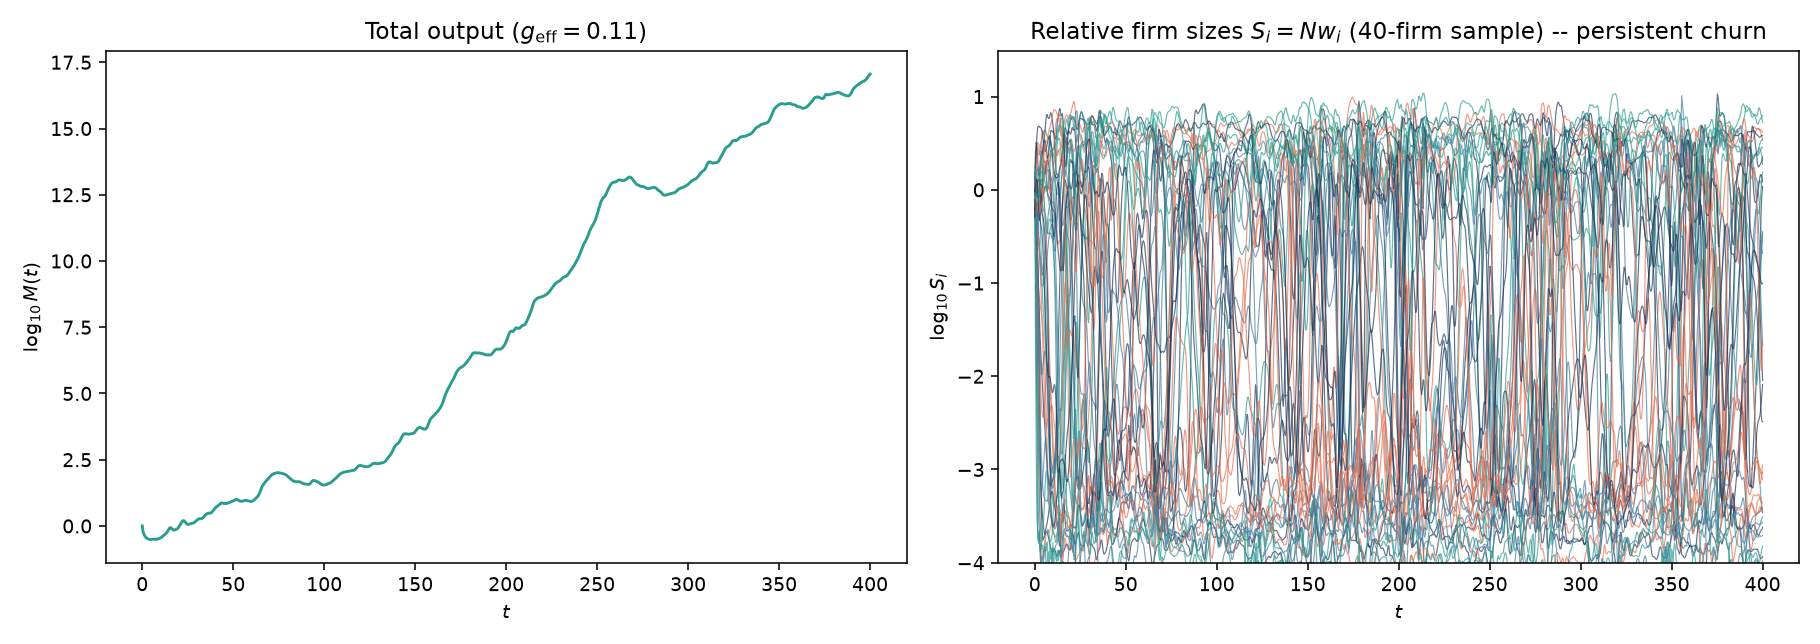
\includegraphics[width=\linewidth]{growing_growth_churn.png}
    \caption{A single run of the relative model \eqref{eq:relative-glv} at $\mu = -1.76$,
    $\sigma = 1.75$, $\lambda = 10^{-3}$ on a power-law graph with $N = 6400$. \panel{Left}: the
    total abundance grows exponentially in physical time, its logarithm rising
    linearly, with no finite-time divergence. \panel{Right}: a sample of relative firm sizes
    $S_i = x_i/m$, which keep fluctuating and exchanging rank rather than relaxing to a
    fixed point.}
    \label{fig:growing-churn}
\end{figure}

\section{Phases of the model}
\label{sec:model-phases}

Before measuring the firm-growth statistics it helps to see where in parameter space the
growing, fluctuating state lives. Figure~\ref{fig:phase-diagram} maps the behaviour of the model
over the plane of the mean interaction $\mu$ and the disorder $\sigma$, classified from the
late-time dynamics of many graph realizations. Two genuine transitions organize it. The
dynamical threshold $\sigma_c$ separates a frozen regime below, where the shape
relaxes to a fixed point and the growth rates vanish, from the chaotic regime above, where it
never settles. Cutting across it, the line $g_{\mathrm{eff}} = 0$ separates a growing economy
from a shrinking one. Where the competition is strong and the disorder high, coexistence
collapses and the dynamics either condense onto a few firms or grow explosively.

The regime we want is pinned down by three things the data demand, and each one rules out part of
the plane. The economy must grow, since output has risen for two centuries, which requires
$g_{\mathrm{eff}} > 0$ and discards the whole shrinking half below the $g_{\mathrm{eff}} = 0$ line.
Its firms must keep growing period after period, so that firm growth is a stationary statistic
rather than a one-off event, and this requires the chaotic phase above $\sigma_c$, since in the
frozen phase below it the shape relaxes to a fixed point and every growth rate vanishes, leaving
the same transient size--variance relation that already ruled out the absolute model. The economy
must also stay diverse, a whole distribution of coexisting firms, which discards the
strong-competition, high-disorder corner where coexistence collapses onto a handful of firms or
the sizes diverge. What survives all three demands is the chaotic, growing band, where the model reproduces the
empirical firm-growth statistics of Moran, Secchi and Bouchaud \citep{moran2024}, the region
labelled MSB in Figure~\ref{fig:phase-diagram}. It is the wedge bounded below by $\sigma_c$, on
the competitive side by the $g_{\mathrm{eff}} = 0$ line, and on the strong-disorder side by the
condensed corner. It is an extended region rather than an isolated point, so what follows
describes the behaviour of the model and not a single tuned operating point.

\begin{figure}[htbp]
    \centering
    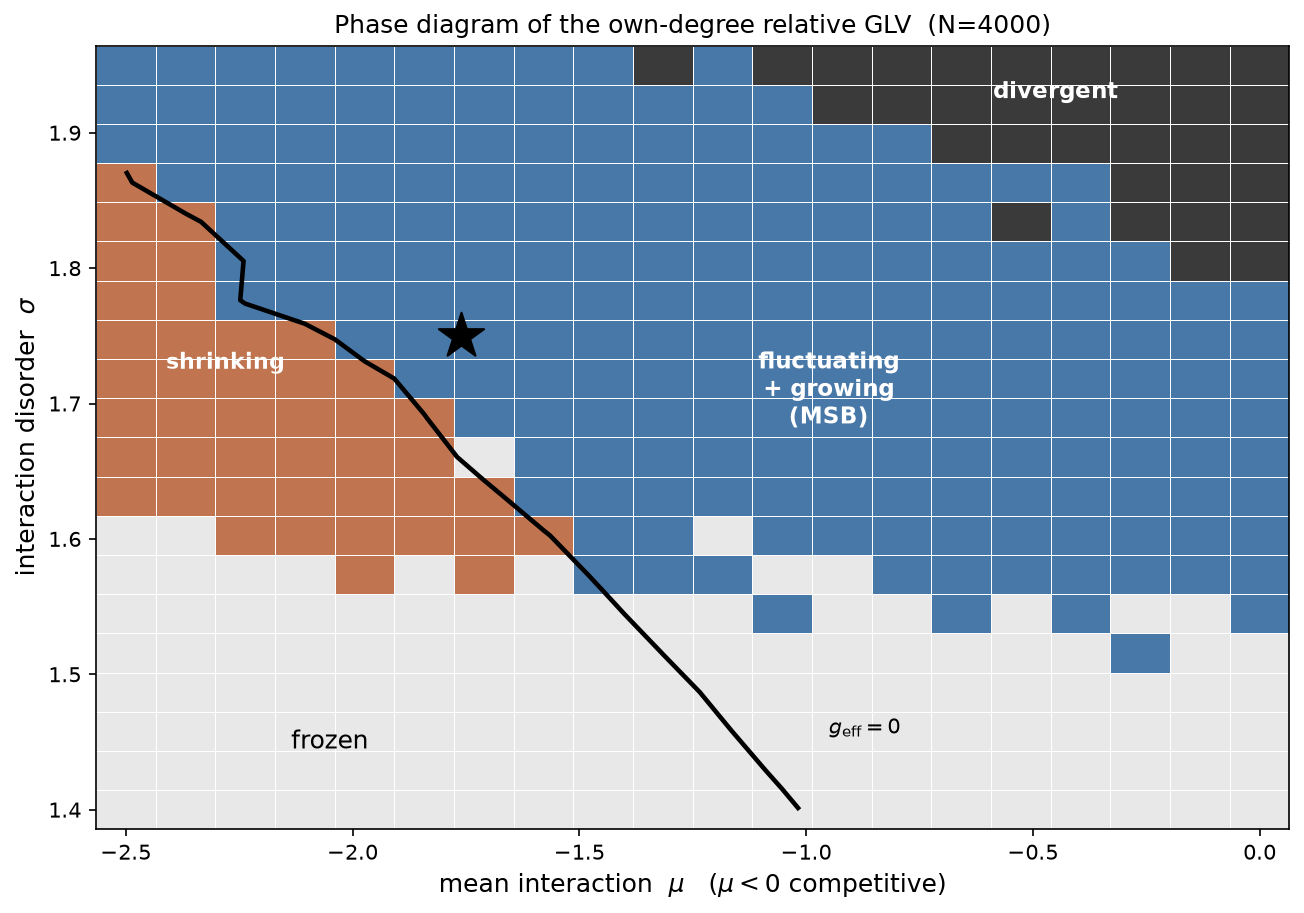
\includegraphics[width=\linewidth]{phase_diagram.png}
    \caption{Phase diagram of the relative model \eqref{eq:relative-glv}, over the mean
    interaction $\mu$ (competitive for $\mu < 0$)
    and the disorder $\sigma$, classified from the late-time dynamics ($N = 4000$, a
    $20 \times 20$ grid with ten realizations per cell). The diagram was mapped under the
    per-firm normalization noted in Section~\ref{sec:completing-model}; under the standard
    normalization used throughout this thesis the same qualitative structure holds but the
    fluctuating band is somewhat narrower --- at the operating point every realization at
    $N \ge 8000$ persists (Chapter~\ref{chap:firmgrowth}), while stronger disorder
    ($\sigma = 2.0$) already loses most realizations to the collapsed corner. At low disorder the shape relaxes and nothing fluctuates
    (frozen). Above it the dynamics are chaotic, and the solid black line marks the growth
    boundary $g_{\mathrm{eff}} = 0$, which separates the shrinking region ($g_{\mathrm{eff}}
    < 0$) from the fluctuating, growing band in which the firm-growth statistics are
    measured (blue, labelled MSB, for Moran--Secchi--Bouchaud). The band is bounded below by the
    freezing line, on the competitive side by $g_{\mathrm{eff}} = 0$, and in the strong-disorder corner by the
    explosive, divergent region. The star marks the operating point $\mu = -1.76$,
    $\sigma = 1.75$. The band is an extended region rather than a single point.}
    \label{fig:phase-diagram}
\end{figure}

This phase structure has a mean-field underpinning. The relative model
\eqref{eq:relative-glv} is a disordered replicator equation, and its dynamical mean-field theory,
worked out in Appendix~\ref{app:dmft}, reduces the $N$-firm dynamics to a single representative
firm in a self-consistent Gaussian field. This is the standard replicator mean-field
\citep{galla2018,roy2020}, whose chaos transition is the mean-field counterpart of the freezing
line. Below it the shape relaxes to a fixed point and the growth rates vanish, above it the flow
never settles. The mean interaction enters every firm's fitness as the same uniform shift, so it
cancels from the replicator and only sets the level of the growth rate $g_{\mathrm{eff}}$, moving
the $g_{\mathrm{eff}} = 0$ line but not the freezing threshold. We locate the threshold and
measure the firm-growth statistics directly from the simulations.

\chapter{Firm-growth statistics}
\label{chap:firmgrowth}

\section{Firm-growth statistics in the fluctuating state}
\label{sec:growing-observables}

We measure the two firm-growth facts on the relative sizes $S_i = x_i/m$ of
Section~\ref{sec:growth-churn}, whose
cross-sectional mean is one by construction. The common growth of the economy is divided
out in the same step, since $\ln S_i = \ln x_i - \ln m$, so the size and its
growth $g_i = \Delta \ln S_i$ are the idiosyncratic part of a firm's trajectory, exactly
what the data measure. As in the empirical protocol, each firm contributes while it
is listed, that is while $S_i$ stays above the immigration floor, and we read growth
rates over a fixed yearly horizon $\Delta t$. All
statistics are taken in a late window, after the initial relaxation has passed, and
restricted to firms that persist across it. They are also taken at $N \ge 8000$: at
smaller sizes the fluctuating state is fragile, and at $N = 2000$ nearly half the graph
realizations collapse onto a fixed point and freeze, while from $N = 8000$ upward every
realization in our ensembles persists.

Two cautions, detailed in Appendix~\ref{app:numerics}, shape the measurement. The
per-firm volatility is a mean-absolute-deviation estimator robust to the fat tails, and
the size--volatility relation is fitted only over its power-law range, the decline above
the small-firm plateau set by the immigration floor. The same appendix varies the
horizon $\Delta t$ and the solver tolerance. The moment ratios are insensitive to both;
$\beta$ is stable for horizons up to the correlation time and drifts upward beyond it,
and the kurtosis falls with the horizon throughout, so the values quoted below refer to
the yearly horizon, as the empirical ones do.

Figure~\ref{fig:growing-msb} shows both observables at the operating point
$\mu = -1.76$, $\sigma = 1.75$ marked in Figure~\ref{fig:phase-diagram}, in the
stationary fluctuating state, for twenty independent economies of $N = 16000$ firms
each. The size--volatility relation (left) falls
monotonically over the fitted range, $\sigma(\bar S) \sim \bar S^{-\beta}$ with a
per-economy exponent
$\beta = 0.45 \pm 0.06$ across realizations. Large firms are less volatile than small ones, as in the
data. The growth-rate distribution (right) is
sharply peaked and fat-tailed, with both flanks heavier than the Laplace reference and
no systematic asymmetry between them (Bowley skewness $+0.01$).

\begin{figure}[htbp]
    \centering
    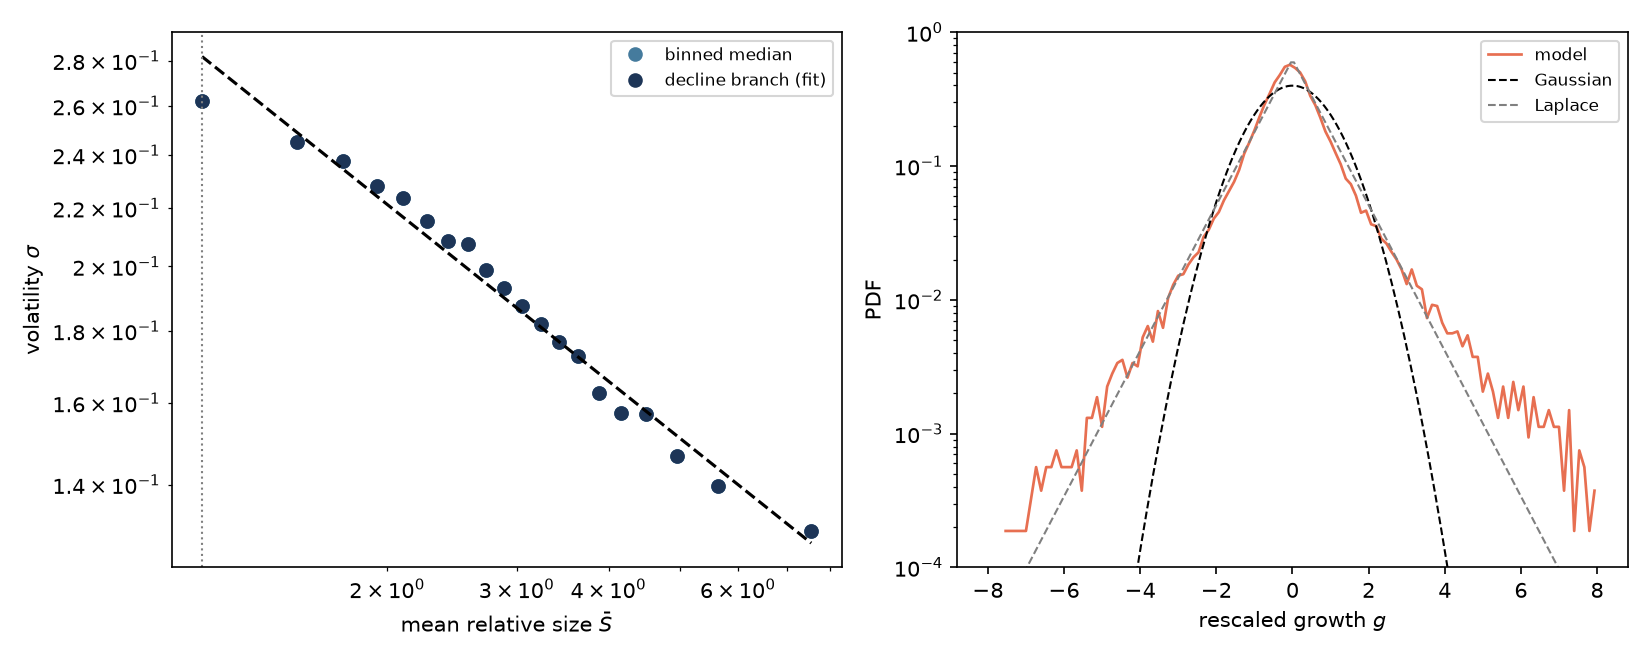
\includegraphics[width=\linewidth]{meandeg_stationary_msb.png}
    \caption{Firm-growth statistics at $\mu = -1.76$, $\sigma = 1.75$, pooled over twenty
    economies of $N = 16000$ firms on the power-law graph
    ($C = 400$, the fixed dilution $C = N/40$). \panel{Left}: the
    size--volatility relation; volatility falls as a
    power law over the fitted decline above the small-firm immigration-floor plateau,
    with per-economy exponent $\beta = 0.45 \pm 0.06$ and $R^2 = 0.99$. \panel{Right}: the
    growth-rate distribution, sharply peaked and fat-tailed,
    heavier than the Laplace reference on both flanks and close to symmetric
    (Bowley $\approx 0$), far above the Gaussian.}
    \label{fig:growing-msb}
\end{figure}

\section{Measuring exponents across realizations}
\label{sec:growing-estimator}

Every exponent in this chapter is measured over many graph realizations, and how the
realizations are combined affects the result. Each economy carries its own
overall volatility scale, set by its particular draw of the couplings, and these scales
differ by large factors from one realization to the next. The obvious estimator pools
the firms of all economies into one sample and fits the size-conditioned moments once.
But conditioning on size across pooled economies then compares a quiet economy's large
firms with a loud economy's small ones, which injects size-independent variance into
every conditional moment. The injected variance flattens the fitted slopes, more
strongly the higher the moment, so the pooled estimator biases every $\zeta_q$ downward,
bends the ratio curve $\zeta_q/\zeta_1$, and the bias does not shrink as more
realizations are added: pooling more economies is not more data for this purpose but
more mixing.

We therefore use the quenched estimator throughout: each exponent is fitted inside a
single economy, on that economy's own decline branch, and the exponents are then
averaged over realizations, with the quoted uncertainty the standard error of that
average. The two estimators disagree materially. At the operating point of
Figure~\ref{fig:growing-msb} the pooled ratios come out $1,\,1.77,\,2.32,\,2.67$ while
the quenched ratios are $1,\,1.84,\,2.51,\,3.02$, a disagreement large enough to
reverse a verdict.
All claims below are therefore quenched, and the pooled values are
reported only for comparison.

\section{Higher moments and the multiscaling}
\label{sec:growing-multiscaling}

The size--variance exponent is only the first moment of a richer object, the distribution
of growth volatility conditional on size, and it is on the higher moments that the
granular models break. \citet{moran2024} measure the $q$-th moment of the
size-conditioned volatility, $E[\sigma^q \mid S] \sim S^{-\zeta_q}$, and find an exponent
that depends on the order $q$: in the data
$\zeta_1,\dots,\zeta_4 \approx 0.20,\,0.39,\,0.51,\,0.58$. Their granular models predict
instead that the three higher moments ``decay with size all with the same scaling'', a
$q$-independent exponent, and it is this prediction the data contradict. As the
introduction set out, two reference lines bound the observable. The granular tail flattens
the ratio curve $\zeta_q/\zeta_1$ to a constant beyond $q=1$; a conditional volatility
with a single scale (a fixed distributional shape whose level alone slides with size)
locks the exponents to the first, $\zeta_q = q\,\zeta_1$, a straight line. The data lie
between them, rising with $q$ but sublinearly, and it is this $q$-dependence, which we
call the multiscaling of the size-conditioned volatility, that a model of firm growth must
reproduce. (\citet{moran2024} read the shortfall below the straight line as a subleading
correction from the incipient tail of their volatility distribution; whether the empirical
sublinearity survives asymptotically is open, and our comparisons are made at the moments
and sizes that are measured.)

Figure~\ref{fig:growing-multiscaling} makes the same measurement in the model, the
first four moments of the size-conditioned volatility, with each economy fitted on
its own decline branch. The quenched exponents rise with the order,
$\zeta_1,\dots,\zeta_4 = 0.41,\,0.76,\,1.03,\,1.24$, with standard errors
$0.01,\,0.03,\,0.04,\,0.05$ over twenty economies; the first is the size--variance
exponent of the previous section. Divided by $\zeta_1$, the
$q$-dependence is $1,\,1.84,\,2.51,\,3.02$ (each $\pm 0.01$--$0.04$), which lies on the
empirical $1,\,2.0,\,2.6,\,2.9$ through $q = 3$ and slightly above it at $q = 4$, and is
separated from the fixed-shape line $\zeta_q/\zeta_1 = q$ by many standard errors at
every $q \ge 2$ (right panel). The ratio curve is converged in system size,
$\zeta_4/\zeta_1 = 3.09,\,3.02,\,3.06$ at $N = 8000$, $16000$, $32000$, and
Appendix~\ref{app:scaling} carries the finite-size study across all topologies. Two
differences in shape remain: the
empirical curve saturates hard after $q = 3$ while the model's bends more gently, so the
model matches the data's values but not its curvature at the highest moment measured;
and the empirical exponents themselves are about half the model's, the magnitude gap
studied in Appendix~\ref{app:scaling}.

\begin{figure}[htbp]
    \centering
    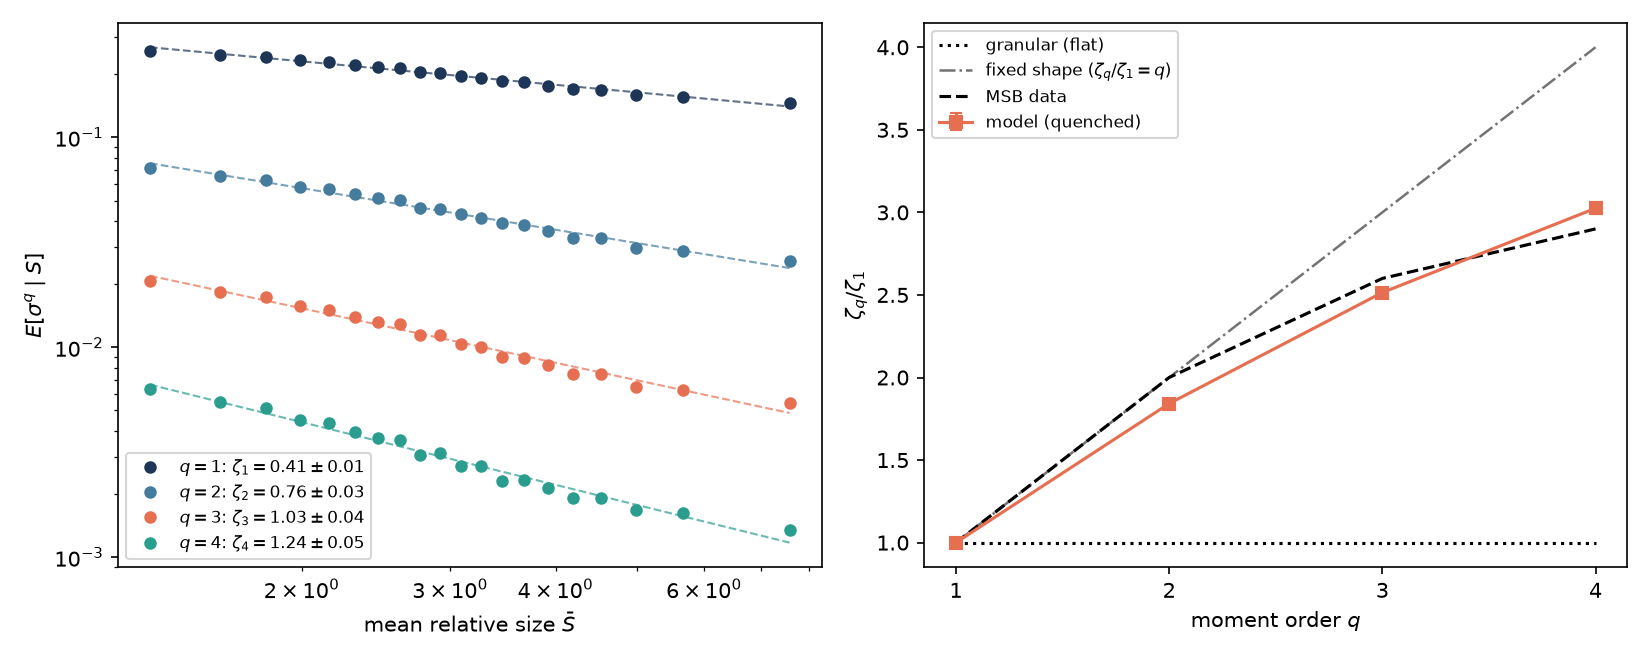
\includegraphics[width=\linewidth]{meandeg_multiscaling.png}
    \caption{Multiscaling of the size-conditioned volatility,
    $\mu = -1.76$, $\sigma = 1.75$, twenty economies of $N = 16000$.
    \panel{Left}: the first four moments $E[\sigma^q \mid S]$
    against mean size on a double-logarithmic scale, each fitted on the decline branch;
    the slopes steepen with the order $q$, the quenched exponents
    $\zeta_1,\dots,\zeta_4 = 0.41,\,0.76,\,1.03,\,1.24$. \panel{Right}: the exponents
    normalized by the first, $\zeta_q/\zeta_1$, against the moment order, for the model,
    the data of \citet{moran2024}, the granular prediction of a $q$-independent
    exponent, and the fixed-shape line $\zeta_q/\zeta_1 = q$ of a conditional volatility
    with a single scale. The model bends below the fixed-shape line onto the empirical
    curve: the shape of the volatility distribution broadens with firm size.}
    \label{fig:growing-multiscaling}
\end{figure}

The multiscaling is the first of three size-conditioned tests by which \citet{moran2024}
separate the data from the granular models, and the model passes the
other two as well (Fig.~\ref{fig:growing-conditional}).

The second asks how the spread of firm volatilities depends on size. Divide each firm's
volatility by the mean volatility at its size, $\sigma_i/\bar\sigma(S)$, and the resulting
distribution should be the same at every size, with a bounded tail. The model reproduces this
collapse onto a single size-independent shape, with a thin tail (the $99$th percentile
sits at $2.2$ times the median when the rescaling is done per economy), and the collapse
tightens, rather than degrading, as the system grows. The granular models predict a
second feature here: large firms built from only a few sub-units keep a fixed volatility that
does not shrink with size, which would show up as a hump in the rescaled distribution.
\citet{moran2024} find no such hump in the data, and the model shows none either; it has no
sub-units to produce one.

The third test turns on the central limit theorem. If a firm
were an aggregate of many independent parts, its growth would look more Gaussian the larger
it grew, so the excess kurtosis of its growth would fall toward zero with size. In the data
the excess kurtosis does not fall with size;
large firms stay at least as fat-tailed as small ones. The model reproduces this: the
excess kurtosis of the size-unmixed growth $(g - \bar g)/\sigma_i$ rises from about two for
the smallest firms to about six for the largest, a trend of $+6.5 \pm 0.5$ per decade of
size measured economy by economy, positive in every one of the twenty realizations. A
firm's growth here is not a
sum of independent contributions, so no central-limit averaging thins its tails as it
grows.

The model thus clears not only the size--variance exponent that the granular models also
fit, but every conditional test by which the data reject them.

\begin{figure}[htbp]
    \centering
    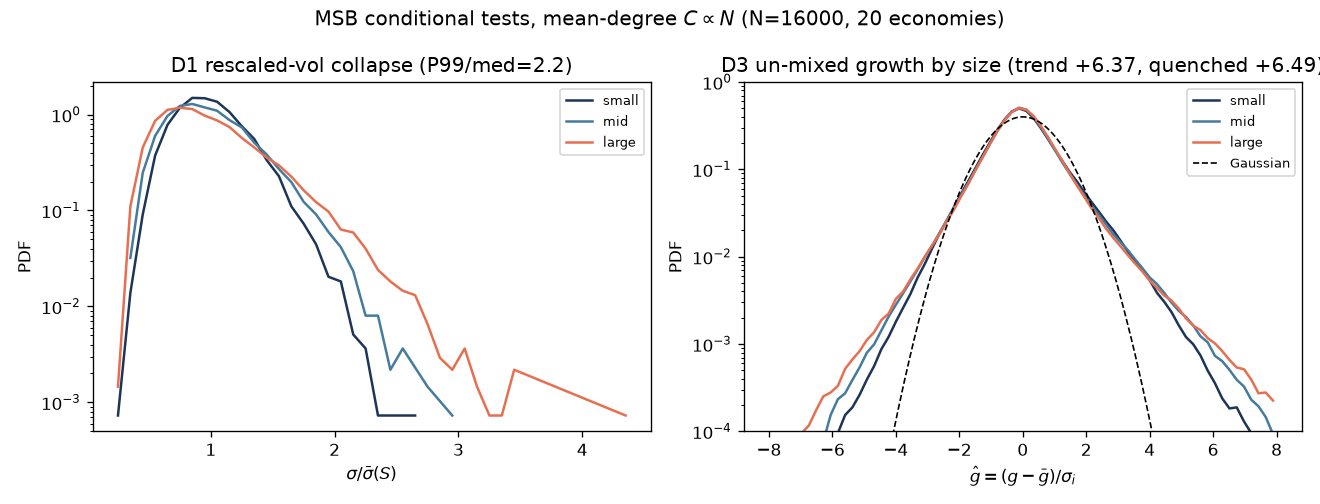
\includegraphics[width=\linewidth]{meandeg_conditional.png}
    \caption{The other two discriminating tests of \citet{moran2024}, twenty economies of
    $N = 16000$. \panel{Left} (second test): the per-firm volatility distribution, rescaled by its
    size-conditional mean $\sigma_i/\bar\sigma(S)$, collapses onto a single size-independent
    shape with a bounded tail. \panel{Right} (third test): the size-unmixed growth $(g-\bar g)/\sigma_i$
    stays fat-tailed at every size, well above the Gaussian, and the larger firms are
    fatter, the excess kurtosis rising with size in every realization; an aggregate of
    independent parts would approach a Gaussian.}
    \label{fig:growing-conditional}
\end{figure}

\section{The role of the graph}
\label{sec:growing-graph}

The couplings put two ingredients into the model, the quenched disorder on the
edges and the heterogeneous degrees of the graph that carries them, and the two can be
separated. Under the standard normalization \eqref{eq:coupling-global} every edge is
divided by the same mean degree, so the variance of the disorder field a firm feels
grows with its own degree, $\mathrm{Var}\,h_i \propto k_i/C$, the same degree-dependent
field that the heterogeneous mean-field theory of \citet{aguirrelopez} carries as a factor
$\sqrt{k_i/C}$ on its noise, so a firm's degree sets the level of noise it feels. If the
multiscaling is really the shape of the volatility distribution broadening with size,
this can produce it, and removing the degree heterogeneity should
then remove the multiscaling as well.

Figure~\ref{fig:growing-topology} repeats the full measurement with only the degree
distribution swapped; the disorder, the operating point and the mean degree $C = N/40$
stay fixed. On the homogeneous graphs the
multiscaling vanishes exactly: the fully-connected control gives ratios
$1,\,2.00,\,3.01,\,4.00$ and the regular graph $1,\,1.99,\,2.95,\,3.87$, the
fixed-shape line to within error. As the degree distribution broadens the ratio curve
bends away from that line, and only the power-law graph with infinite degree variance
(exponent $2.5$, the graph of every other figure in this chapter) reaches the empirical
curve. The size--variance exponent moves with the same parameter, from $\beta \approx 1$ on
the homogeneous graphs down through $0.73$ (power-law $3.5$) and $0.43$ (power-law $2.5$)
to $0.17$ (power-law $2.2$), inside the empirical band at this size:
degree heterogeneity is what pushes the exponent down toward, and through, the empirical
range. The tail exponent of the graph is thus a single control parameter that carries both
size-conditioned observables across the empirical values: the data are bracketed
between exponent $2.2$, where $\beta$ is right and the ratios run slightly low, and
$2.5$, where the ratios are right and $\beta$ is high. Pushing the tail harder still
(exponent $2.1$ and below) overshoots: $\beta$ falls below the band while half the
realizations freeze and the ratio measurement degrades, so the empirical pair sits at
the heterogeneous but still stable edge of the family. The
growth tent, by contrast, is indifferent to all of it, fat and symmetric on every
topology including the fully-connected one, so the tent belongs to the disorder alone
while the size-conditioned structure belongs to the graph.

The power-law-$2.2$ graph, the bracketing partner that carries the empirical exponent,
passes the full battery of conditional tests as well. Run at the same operating point
and size as the headline measurements ($N = 16000$, twenty economies, all surviving),
it gives $\beta = 0.21 \pm 0.07$, inside the empirical band at a size where
Appendix~\ref{app:scaling} shows this exponent converged; quenched ratios
$1,\,1.79,\,2.36,\,2.72$, tracking the empirical curve from below; a
rescaled-volatility collapse as tight as the headline graph's (tail $P_{99}$/median
$2.0$ against $2.0$ at exponent $2.5$, with size-independent medians); a size-unmixed
kurtosis rising with size at $+5.8 \pm 0.6$ per decade, positive in nineteen of the
twenty economies; and a symmetric fat tent (Bowley $+0.02$, excess kurtosis $10.5$).
The two bracketing exponents therefore fail in different places and by very different
margins: at $2.2$ the worst deviation is the highest ratios running $5$--$7\%$ below
the data, while at $2.5$ the ratios sit on the data but the exponent overshoots the
empirical band by a factor of two and is still drifting. Every conditional test is
passed at both.

\begin{figure}[htbp]
    \centering
    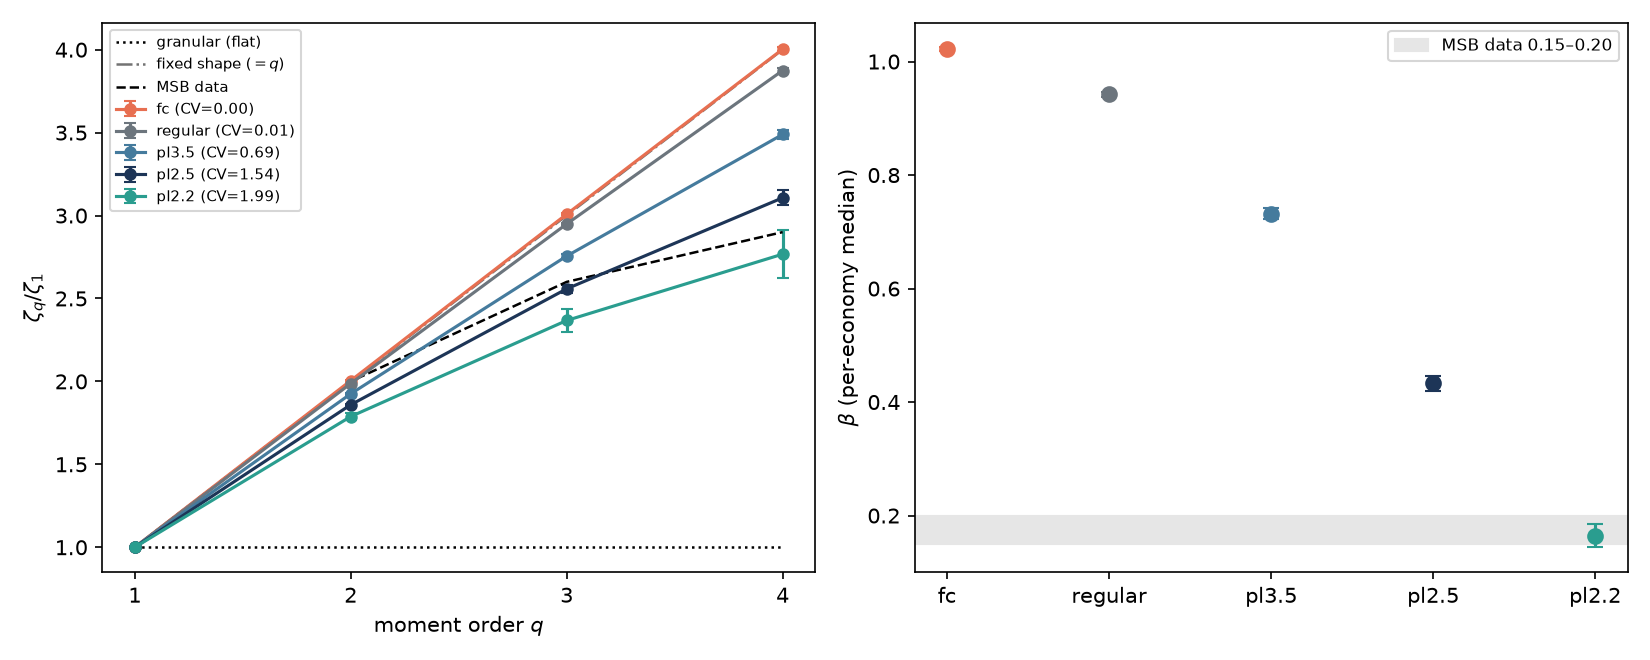
\includegraphics[width=\linewidth]{meandeg_topology.png}
    \caption{The graph generates the size-conditioned statistics. Five degree
    distributions at the same operating point, mean degree and disorder, twenty economies
    each ($N = 8000$; the ordering is unchanged at $N = 16000$). \panel{Left}: quenched
    multiscaling ratios. The homogeneous graphs (fully connected, regular) sit on the
    fixed-shape line $\zeta_q/\zeta_1 = q$ (no multiscaling) and the curve bends
    toward the data as the degree distribution broadens (CV is the coefficient of
    variation of the degrees); only the infinite-variance power-law graphs reach the
    neighbourhood of the empirical curve. \panel{Right}: the size--variance exponent falls from $\beta \approx 1$
    on homogeneous graphs toward the empirical range as heterogeneity grows.
    Table~\ref{tab:growing-topology} gives the numbers.}
    \label{fig:growing-topology}
\end{figure}

\begin{table}[htbp]
    \centering
    \begin{tabular}{lcccccc}
        \hline
        graph & survive & $\beta$ & $\zeta_2/\zeta_1$ & $\zeta_3/\zeta_1$
              & $\zeta_4/\zeta_1$ & tent exkurt \\
        \hline
        fully connected & $20/20$ & $1.02$ & $2.00$ & $3.01$ & $4.00$ & $11$ \\
        regular         & $20/20$ & $0.94$ & $1.99$ & $2.95$ & $3.87$ & $11$ \\
        power law $3.5$ & $20/20$ & $0.73$ & $1.93$ & $2.76$ & $3.49$ & $8$  \\
        power law $2.5$ & $20/20$ & $0.43$ & $1.86$ & $2.56$ & $3.11$ & $8$  \\
        power law $2.2$ & $20/20$ & $0.17$ & $1.79$ & $2.37$ & $2.77$ & $9$  \\
        \hline
        fixed shape     &         &        & $2$    & $3$    & $4$    &      \\
        MSB data        &         & $0.15$--$0.20$ & $2.0$ & $2.6$ & $2.9$ &  \\
        \hline
    \end{tabular}
    \caption{The topology sweep of Figure~\ref{fig:growing-topology} in numbers: the same
    operating point, disorder and mean degree, only the degree distribution swapped
    ($N = 8000$, twenty realizations per graph). $\beta$ is the median per-economy
    decline-branch slope (standard errors $0.003$--$0.020$); the ratios are quenched means
    over economies (standard errors $\le 0.05$, the power-law-$2.2$ ratios up to
    $0.14$); the tent excess kurtosis
    is the per-economy median. Homogeneous graphs sit on the fixed-shape row to within
    error, the power-law-$2.5$ graph approaches the empirical ratio row, and the
    power-law-$2.2$ graph places $\beta$ inside the empirical band at this size with
    ratios slightly below the data; the growth
    tent stays fat on every topology. (An exponential-degree graph at the same operating
    point sits at the edge of the freezing transition, losing a third of its realizations,
    and is omitted.)}
    \label{tab:growing-topology}
\end{table}

This ablation is the counterpart of a second one, on the disorder itself.
Table~\ref{tab:growing-ablation} sweeps $\sigma$ at fixed $\mu$, $\lambda$
and $N$. Below the threshold $\sigma_c$ the dynamics freeze: the late-time
growth fluctuations are zero to the precision quoted, the shape has relaxed to a fixed
point, and there is no fluctuating state to measure. The persistent fluctuations and
the fat-tailed tent appear only once $\sigma$ crosses $\sigma_c$, growing with the
disorder. With no noise in the model, the fluctuations can come only from the disorder,
and removing it removes them entirely. The two ablations together assign the phenomena
to their sources: the disorder makes the economy fluctuate and gives the growth
distribution its heavy tails; the degree heterogeneity of the graph turns those
fluctuations into the size-conditioned structure (the low exponent and the
multiscaling) that the data show.

\begin{table}[h]
    \centering
    \begin{tabular}{rccc}
        \hline
        $\sigma$ & growth fluctuation & excess kurtosis & fat-tailed tent? \\
        \hline
        $0.00$ & $0.000$ & --   & no  \\
        $0.50$ & $0.000$ & --   & no  \\
        $1.00$ & $0.000$ & --   & no  \\
        $1.41$ & $0.000$ & --   & no  \\
        $1.60$ & $0.085$ & $14$ & yes \\
        $1.75$ & $0.175$ & $14$ & yes \\
        \hline
    \end{tabular}
    \caption{Disorder ablation at $\mu = -1.76$, $\lambda = 10^{-3}$, $N = 3200$ on a
    power-law graph. ``Growth fluctuation'' is the standard deviation of the pooled
    late-window growth rates. Below the chaotic threshold $\sigma_c$ the state
    freezes (growth fluctuation zero to the precision quoted) and there is no genuine
    fluctuating distribution to characterize, so the kurtosis is left blank; the
    persistent fluctuations and the fat-tailed tent switch on only once $\sigma$ crosses
    $\sigma_c$. (A nonzero $\beta$ can still be fitted below threshold. It reflects a frozen
    state during its relaxation, the V transient of the absolute critical model, and says
    nothing about a stationary fluctuating law.)}
    \label{tab:growing-ablation}
\end{table}

The interactions-only origin also separates this model from the simplest alternatives. A
mean-field multiplicative model with injected noise already gives a growing economy with a
stationary heavy-tailed size distribution \citep{bouchaudmezard2000}, but there the
fluctuations are external and there is no network. Here the same growing aggregate, the heavy tails,
and the slow size--variance decay arise together from the disordered
interactions, and the size-conditioned structure from the topology that carries them.

\section{From degree to size: survival under competition}
\label{sec:growing-degree-size}

The degree-dependent field variance that carries the graph into the statistics also
acts on the individual firm, and its effect has two parts: degree sets size but barely
touches volatility, and it sets size not by advantaging the connected firm but by
widening the spread of outcomes among connected firms, most of which lose.

The first part is the observation itself, shown in Fig.~\ref{fig:growing-degree-size}.
Measured per economy at the operating point, a firm's mean size rises with its degree, Spearman
correlation $+0.41$ (range $+0.37$ to $+0.44$ across ten economies of $N = 16000$),
positive in every realization, and the relation is a power law,
$\bar S \sim k^{\delta}$ with $\delta = 0.56 \pm 0.02$. Unlike the size--variance
exponent, $\delta$ is converged at our sizes: it is $0.57 \pm 0.03$ at $N = 8000$ and
unchanged at $N = 16000$. The firm's volatility, by contrast, is nearly flat in its
degree (Spearman $+0.16$, right panel), and the flatness is a near-cancellation of two
opposing dependences. Fitted jointly across the firms of twelve economies at
$N = 8000$, the volatility scales as $\sigma_i \propto k_i^{\,b}\,\bar S_i^{-a}$ with
$b = 0.486 \pm 0.012$ and $a = 0.588 \pm 0.015$: at fixed size a hub is noisier, the
$k_i/C$ field variance of Section~\ref{sec:growing-graph} surfacing directly, but the
size that noise procures quiets the firm through the size--variance law, and the two
compose to $\sigma \propto k^{\,b - a\delta} \approx k^{+0.16}$ with $\delta = 0.56$,
the weak residual the figure shows. Degree acts on size, and the
volatility inherits only what the size--variance law leaves over.

\begin{figure}[htbp]
    \centering
    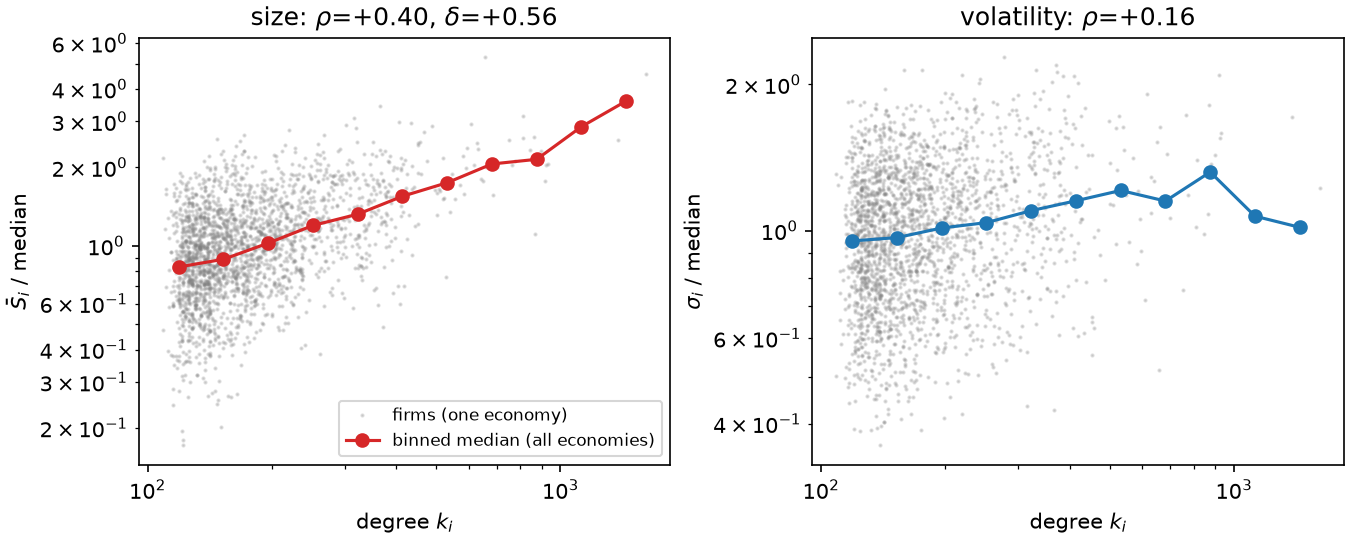
\includegraphics[width=\linewidth]{meandeg_degree_size.png}
    \caption{Degree and the individual firm, ten economies of $N = 16000$ ($C = 400$),
    each economy's sizes and volatilities normalized by its own median. \panel{Left}:
    mean size against degree; the binned median (across all economies) rises as a power
    law $\bar S \sim k^{\delta}$, $\delta = 0.56 \pm 0.02$, per-economy Spearman
    correlation $+0.41$. \panel{Right}: volatility against degree is nearly flat
    (Spearman $+0.16$): the two opposing degree dependences, the noise rising with
    degree and the size it procures quieting the firm, nearly cancel, and
    $\sigma \sim k^{+0.16}$ is the residual.}
    \label{fig:growing-degree-size}
\end{figure}

The second part is the selection behind the relation. Under competition ($\mu < 0$) a
hub has more competitors and feels a mean suppression that grows with its connectivity,
and most hubs indeed lose: the survival probability falls monotonically with degree,
from $0.22 \pm 0.05$ in the lowest degree bin to $0.02 \pm 0.02$ in the highest. A
firm's couplings are also a quenched draw whose spread widens with degree, and
conditioning on survival reverses the correlation between the average interaction field
a firm sits in and its degree, from $-0.27$ over all firms to $+0.35$ among the
survivors, so the hubs that remain are those whose draw came out favourable, and their
sizes track those favourable fields. The field the survivors are drawn from is
fat-tailed, a sum over neighbours weighted by their heavy-tailed sizes, and the largest
survivors live in exactly that tail.

A final control assigns the diversity itself to the competition. Setting $\mu = 0$ at
the same disorder removes the mean suppression, and with it the coexistence: the
economy condenses onto a handful of firms (survival below $0.2\%$ in every
realization), so the same penalty that eliminates the typical hub holds the rest of the
economy in coexistence. Connectivity widens the quenched draw a firm receives,
competition removes most of the widened draws, and the surviving tail is large in
proportion to the widening. As in Section~\ref{sec:growing-graph}, the firm-to-firm
structure is quenched, frozen into the realized couplings, and the dynamics select and
expose it.

\chapter{Conclusion}
\label{chap:conclusion}

This thesis asked whether a dynamical model of interacting firms can produce the
firm-growth anomalies by itself, without the heavy-tailed internal composition that the
granular models assume and that \citet{moran2024} show the data reject. A Generalized
Lotka--Volterra network whose firms are identical, with no injected
noise and no built-in correlations, recovers the fat-tailed growth-rate distribution, a
size--variance relation that decreases with firm size, as in the data, and every size-conditioned
test by which the data reject the granular picture: the anomalous multiscaling of the
higher volatility moments, the collapse of the rescaled volatility distribution with a
bounded tail, and the persistence of fat tails in the growth of the largest firms. All
come out as stationary properties of an economy that grows while its composition keeps
fluctuating.

The model is one change to the standard Generalized Lotka--Volterra system.
Self-limitation and interactions act on a firm's size relative to the average firm rather
than on its absolute size, which makes the dynamics scale-invariant. Total output then grows
exponentially, without the finite-time blow-up of the absolute model, and in the strongly
disordered regime the composition of the economy never settles but keeps fluctuating
chaotically. The couplings use the standard Lotka--Volterra normalization of the disordered
literature, on a scale-free graph whose mean degree scales with the
number of firms.

The results point to two distinct mechanisms.
Switching the disorder off and on shows the fluctuations and the fat-tailed growth
distribution to be made by the disordered interactions; they appear on every topology,
including a fully connected one. Swapping the degree distribution of the graph, with
everything else held fixed, shows the size-conditioned structure (the low
size--variance exponent and the multiscaling) to be made by the degree heterogeneity.
Under the standard normalization a firm's noise variance grows with its connectivity, so
the graph's degree distribution sets the distribution of noise levels across firms. On
homogeneous graphs the multiscaling vanishes exactly; as the degree distribution
broadens the ratio curve bends toward the data, and only the scale-free graph reaches
it. The same heterogeneity reaches the individual firm through survival: most highly
connected firms are driven to the immigration floor, and the survivors'
sizes grow with degree as $\bar S \sim k^{0.56}$, so the degree hierarchy shapes
the size hierarchy as well as the noise.
A network account of the \emph{level} of firm volatility, resting on customer
concentration, already exists \citep{herskovic2020}; the present model adds that the
\emph{size-conditioned} statistics follow from the heterogeneity of the interaction
graph.

Three limitations are important. First, neither the dynamics nor the construction is new,
and Chapter~\ref{chap:background} places both in their lineage: the fluctuating
regime is the chaotic phase of the disordered Lotka--Volterra model \citep{diederich1989,bunin2017,galla2018,roy2020},
and the scale invariance and mean-coupling are those of the econophysics models of wealth and
firm sizes \citep{bouchaudmezard2000,malcai2002}. What is
specific here is the combination, self-limitation and disordered interactions made relative
together, and the finding that the graph's heterogeneity generates the discriminating
firm-growth statistics. Second,
the quantitative match is partial. The
multiscaling ratios and the conditional tests (the shape of the size-conditioned
statistics) are reproduced and are converged in system size. The absolute scale is
not on the same graph: on the power-law-$2.5$ graph of the headline figures the
size--variance exponent stands at $\beta \approx 0.45$ at $N = 16000$ and
$0.49$ at $N = 32000$,
against the empirical $0.15$--$0.20$, still drifting slowly upward, while on the
power-law-$2.2$ graph the exponent is converged at the upper edge of the empirical band
($\beta \approx 0.21$--$0.23$) with the multiscaling ratios then running
$5$--$7\%$ below the data; no single tail exponent yet places both on the data at
once. The model robustly predicts the shape of the statistics, while their scale remains a finite-size
quantity. Third,
the growth is near-critical: the operating point sits in the growing band but not far
from its boundaries; stronger disorder loses realizations to collapse, and a
lighter-tailed graph pushes them into freezing. Perturbing the operating point
($\sigma$ from $1.5$ to $2.0$, $\mu$ from $-1.4$ to $-2.1$) moves the size--variance
exponent substantially ($\beta = 0.28$--$0.79$) while the ratio curve stays bent below
the fixed-shape line wherever the fluctuating state survives, so the multiscaling is a
property of the phase and the particular exponent values of the operating point.

\enlargethispage{\baselineskip}
The exponent's slow upward drift calls for determining its limiting value and for developing an analytical
theory. The mean-field treatment of Appendix~\ref{app:dmft} stops at the relaxed phase
on the homogeneous graph. The
size distribution, measured in Appendix~\ref{app:size-distribution}, is effectively
truncated where the data are Zipf-like, so matching it will take a modified model, not a
larger simulation.
The immigration floor's plateau on the smallest firms is worth a second look,
now that \citet{fontanelli2025} report an empirical size--volatility relation
that steepens for small firms and flattens for large ones.
The correlation structure is the sharper question. \citet{moran2024} conjecture that
the granular models fail for lack of a between-firm growth correlation that grows
with size; Appendix~\ref{app:correlations} measures that correlation directly and finds it modest
and roughly independent of both size and degree. The model therefore reproduces the
size-conditioned statistics through the degree-dependence of the noise amplitude, not
through the size-dependent correlations proposed by Moran et al. Whether real firms
carry the size-growing or the flat correlation is a question for firm-level data on a
known network. Incorporating couplings from real input--output and supply linkages would connect the model
more directly to the macroeconomic dynamics behind these stylized facts.


\vspace{100pt}

\printbibliography

\appendix
\chapter{Dynamical mean-field theory of the relative model}
\label{app:dmft}
\providecommand{\Dz}{\mathcal{D}z}
\providecommand{\E}{\mathbb{E}}

This note derives a dynamical mean-field theory (DMFT) for the scale-invariant model of
the growing-economy chapter, in which the interactions act on the average firm rather
than on absolute abundances. The model turns out to be a disordered replicator equation,
so its DMFT is the heterogeneous single-site process already used to locate $\mu_c$
\citep{aguirrelopez}, with two small additions that the scale invariance forces. The
reduction to a replicator and the resulting effective single-site process and its
self-consistency conditions are set out below.

\section{The model and its reduction to a replicator}
\label{sec:dmft-model}

We take the relative GLV in the competition convention used in the simulations,
\begin{equation}
    \dot x_i = x_i\left[\,1 - \frac{x_i}{m} - \frac{(\alpha x)_i}{m}\,\right],
    \qquad m = \frac1N\sum_j x_j = \frac MN ,
    \label{eq:dmft-glv}
\end{equation}
with couplings on a graph of mean degree $C$,
\begin{equation}
    \alpha_{ij} = A_{ij}\Big(-\frac{\mu}{C} + \frac{\sigma}{\sqrt C}\,z_{ij}\Big),\qquad
    z_{ij}\sim\mathcal N(0,1),\qquad \overline{z_{ij}z_{ji}} = \gamma,\qquad \alpha_{ii}=0 .
\end{equation}
Both the self-limitation $x_i/m$ and the interaction $(\alpha x)_i/m$ are divided by the
population mean $m$. The right-hand side of \eqref{eq:dmft-glv} is then homogeneous of
degree one in $x$, so the bracket $F_i := 1 - x_i/m - (\alpha x)_i/m$ depends on $x$ only
through ratios. The overall scale is a free direction that grows or decays exponentially
without the finite-time blow-up of the absolute model.

Introduce the relative abundances $y_i = x_i/m$, which satisfy $\langle y\rangle :=
\frac1N\sum_i y_i = 1$ by construction, and let $M = \sum_j x_j$ be the total. The
aggregate grows at the population-averaged fitness,
\begin{equation}
    g(t) := \frac{d\ln M}{dt}
          = \frac1M\sum_j \dot x_j = \sum_j \frac{x_j}{M}\,F_j
          = \frac1N\sum_j y_j F_j = \langle yF\rangle .
    \label{eq:dmft-g}
\end{equation}
Subtracting this common scale leaves a closed equation for the relative abundances,
\begin{equation}
    \dot y_i = y_i\big(F_i - g(t)\big),\qquad
    F_i = 1 - y_i - (\alpha y)_i,\qquad
    g(t) = \langle yF\rangle ,
    \label{eq:dmft-replicator}
\end{equation}
which is a replicator equation, the simplex projection of \eqref{eq:dmft-glv} in the sense
of Hofbauer's correspondence \citep{hofbauer81}. The aggregate is recovered from
$M(t) = M(0)\exp\!\int_0^t g$, and a positive stationary $g$ is a steadily growing
economy.

\paragraph{What the $-g(t)$ term is.}
The drift $-g(t)$ in \eqref{eq:dmft-replicator} is the mean-fitness subtraction of the
replicator, and it is the term that turns the equation for absolute size into one for
relative size. From \eqref{eq:dmft-g}, $g(t) = \langle yF\rangle = \sum_j w_j F_j$ is the
share-weighted average fitness of the whole economy, with shares $w_j = y_j/N = x_j/M$,
and it equals the growth rate of the aggregate, $g(t) = d\ln M/dt$. Every firm feels the
same $g(t)$. It is a global field common to all firms rather than something private to firm $i$. A firm therefore
gains relative size, $\dot y_i > 0$, only when its own fitness $F_i$ exceeds the
economy-wide average $g(t)$, so $-g(t)$ encodes the requirement to beat the field in
order to gain ground. Its role is to enforce the constraint $\langle y\rangle = 1$. One
checks from \eqref{eq:dmft-replicator} that $\frac{d}{dt}\langle y\rangle = \langle
yF\rangle - g\langle y\rangle = g\,(1 - \langle y\rangle)$, so $\langle y\rangle = 1$ is
preserved, and $g(t) = \langle yF\rangle$ is precisely the value that keeps it preserved.
Because it is an average over the whole population, $g(t)$ self-averages. Its fluctuations
are of order $1/\sqrt N$ and vanish in the thermodynamic limit, so it enters the mean-field
description as a deterministic common drift rather than as a source of noise.

\section{The local field and the effective single-site process}
\label{sec:dmft-cavity}

We take the high-connectivity limit and treat the regular graph, so that
$k_i \equiv C$. Split the interaction felt by node $i$ into its mean and
its fluctuation,
\begin{equation}
    (\alpha y)_i
    = -\frac{\mu}{C}\sum_{j\in\partial i} y_j + \frac{\sigma}{\sqrt C}\sum_{j\in\partial i} z_{ij} y_j
    \;\longrightarrow\; -\mu M_1(t) + h_i(t),
\end{equation}
where the neighbourhood average of the mean part tends to the global one, $-\mu M_1$ with
$M_1 = \langle y\rangle$, and $h_i$ collects the disorder. The dynamical cavity argument
\citep{bunin2017,galla2018} proceeds by removing node $i$. The cavity trajectories
$y_j^{(i)}$ are independent of the couplings $\{z_{ij}, z_{ji}\}$, and reinstating $i$
perturbs each neighbour by linear response. The field that $i$ exerts on $j$ has
fluctuating part $-\frac{\sigma}{\sqrt C} z_{ji} y_i$, so with the single-site response
$G_j(t,s) = \delta y_j(t)/\delta\zeta_j(s)$,
\begin{equation}
    h_i(t)
    = \frac{\sigma}{\sqrt C}\sum_{j\in\partial i} z_{ij}\,y_j^{(i)}(t)
    \;-\; \frac{\sigma^2}{C}\sum_{j\in\partial i} z_{ij}z_{ji}\!\int_0^t\! ds\,G_j(t,s)\,y_i(s).
\end{equation}
The first sum is a sum of $C$ independent zero-mean terms; by the central limit theorem it
becomes a Gaussian noise $\xi_i(t)$ whose covariance is the population autocorrelation,
\begin{equation}
    \langle\xi_i(t)\xi_i(s)\rangle
    = \frac{\sigma^2}{C}\sum_{j\in\partial i} y_j(t)y_j(s)
    = \sigma^2\,C(t,s),\qquad C(t,s):=\langle y(t)y(s)\rangle .
\end{equation}
The second sum uses $\overline{z_{ij}z_{ji}} = \gamma$ and
$\frac1C\sum_{j\in\partial i} G_j \to G := \langle G_j\rangle$, giving the retarded Onsager
reaction $-\gamma\sigma^2\!\int_0^t G(t,s)\,y_i(s)\,ds$. Substituting into $F_i = 1 - y_i +
\mu M_1 - h_i$ and using \eqref{eq:dmft-replicator} produces the effective single-site
process
\begin{equation}
    \boxed{\;
    \dot y = y\left[\,1 - y + \mu M_1(t) - g(t)
        + \sigma\,\eta(t) + \gamma\sigma^2\!\int_0^t\! G(t,s)\,y(s)\,ds\,\right],
    \;}
    \label{eq:dmft-singlesite}
\end{equation}
with $\eta$ a unit-strength Gaussian noise of covariance $\langle\eta(t)\eta(s)\rangle =
C(t,s)$. Equation~\eqref{eq:dmft-singlesite} is the heterogeneous effective process of
\citet{aguirrelopez} with carrying capacity $K=1$, the competition sign on the mean field,
and the two structural additions forced by the scale invariance, namely the common drift $-g(t)$
of Section~\ref{sec:dmft-model}, and the constraint that the mean abundance is pinned,
$M_1\equiv 1$, rather than left free.

\section{Self-consistency}
\label{sec:dmft-selfconsistency}

The disorder average is now carried by four functionals of the single-site law of
\eqref{eq:dmft-singlesite}:
\begin{equation}
    M_1(t) = \E[y(t)] = 1,\qquad
    C(t,s) = \E[y(t)y(s)],\qquad
    G(t,s) = \E\!\left[\frac{\delta y(t)}{\delta\zeta(s)}\right]_{\zeta=0},
\end{equation}
\begin{equation}
    g(t) = \E[y(t)F(t)],\qquad
    F = 1 - y + \mu M_1 + \sigma\eta + \gamma\sigma^2\!\int_0^t G\,y .
    \label{eq:dmft-closures}
\end{equation}
The first is the normalisation, the middle two are the standard correlation and response
that close the noise and the memory, and the last fixes the common drift. The closure for
$g$ is forced rather than chosen. We have $\dot M_1 = \E[yF] - g M_1$, and demanding $\dot M_1 = 0$
at $M_1 = 1$ gives $g(t) = \E[yF]$. This has the structure of a solvable random-replicator
model, here carrying the GLV self-limitation as well. Solving these self-consistency
conditions is the standard replicator mean-field problem \citep{galla2018,roy2020}; the
freezing threshold is taken from simulation in the main text. What the single-site
process does deliver analytically is the structure of the size--volatility statistics,
set out next.


\section{From the single-site process to the size--volatility statistics}
\label{sec:dmft-beta}

The couplings of the simulations are fully asymmetric, $\gamma = 0$, so the memory term
of \eqref{eq:dmft-singlesite} drops and the single-site process in log-size reads
\begin{equation}
    \frac{d\ln y}{dt} = A(t) - y,
    \qquad A(t) = 1 + \mu - g(t) + \sigma\,\eta(t),
    \label{eq:dmft-logprocess}
\end{equation}
with $\eta$ the self-consistent Gaussian field, correlated over the churn time
$\tau_c = O(1)$ of the population autocorrelation ($y$ here is the relative size, the
$S$ of the main text). The three ingredients of what follows --- a self-limitation whose
restoring rate grows with the abundance, a coloured field of finite correlation time, and
a floor that keeps the smallest firms alive --- are those of the fluctuating-phase
single-species process studied by \citet{arnouxbunin2024}, and the damping of the most
abundant species by their own self-limitation is the effect \citet{mallmin2024} describe
in the chaotic turnover regime. What we add is the consequence for the size-conditioned
volatility. Conditional on a firm's window-averaged level $\bar y$, the
fluctuations of $\ln y$ obey an Ornstein--Uhlenbeck equation whose damping rate is
$\bar y$ itself --- the self-limitation stiffens with size --- driven by a noise whose
amplitude does not depend on the level. Two regimes follow. Small firms,
$\bar y\,\tau_c \ll 1$, relax more slowly than the field varies, and the variance of
their growth over a fixed horizon is level-independent: a plateau. Large firms,
$\bar y\,\tau_c \gg 1$, track the fluctuating field adiabatically, $\delta y \sim
\sigma\,\delta\eta$ whatever the level, so $\delta\ln y \propto 1/\bar y$ and
\begin{equation}
    \sigma_{\mathrm{vol}}(\bar y) \propto \bar y^{-1}:
    \qquad \beta_{\mathrm{hom}} = 1,
\end{equation}
with the knee between the two regimes at $\bar y \sim 1/\tau_c \approx 1$. Both
predictions are borne out on the homogeneous graphs of
Section~\ref{sec:growing-graph}: the measured exponents are $1.02 \pm 0.003$ (fully
connected) and $0.94 \pm 0.004$ (regular), and the plateau--decline knee sits at
$\bar S \approx 1$ in every size--volatility figure.

The same argument fixes the higher moments on a homogeneous graph. The single-site
process carries one noise scale, so conditional on the level the volatility is
deterministic, $E[\sigma^q \mid \bar y] = \sigma_{\mathrm{vol}}(\bar y)^q$, and every
moment is a power of the first:
\begin{equation}
    \zeta_q = q\,\zeta_1
\end{equation}
exactly, whatever the local slope. This is the fixed-shape line of the main text, and
it is a parameter-free prediction: the fully-connected control measures
$\zeta_q/\zeta_1 = 1,\,2.00,\,3.01,\,4.00$ and the regular graph
$1,\,1.99,\,2.95,\,3.87$ (Table~\ref{tab:growing-topology}). The mean-field theory
thus accounts quantitatively for the homogeneous rows of that table, and locates the
empirical statistics in the departure from it.

On the heterogeneous graph the departure enters through one channel. The noise a firm
feels is its own neighbourhood sum, of variance
$(\sigma^2/C)\sum_{j\in\partial i} y_j^2 \propto k_i/C$; this is the degree-dependent
amplitude $\sqrt{k_i/C}$ that \citet{aguirrelopez} carries through the heterogeneous
mean-field theory, there evaluated at the fixed points of the non-growing model. Applying
the single-site argument firm by firm with that amplitude predicts the bridge law
\begin{equation}
    \sigma_i \;\propto\; k_i^{1/2}\; \bar y_i^{\,-a},
    \label{eq:dmft-bridge}
\end{equation}
with $a$ the effective damping exponent over the fitted range ($a = 1$ in the
adiabatic limit). A bivariate fit across the firms of twelve economies at $N = 8000$
gives $b = 0.486 \pm 0.012$ for the degree exponent, confirming the predicted
$\tfrac12$ with no adjustable parameter, and measures $a = 0.588 \pm 0.015$ --- the
fitted decade $\bar S \sim 1$--$10$ straddles the plateau--adiabatic crossover, so the
effective damping exponent sits below its asymptotic value; it is a measured quantity
here, not a derived one.

The bridge law converts the size-conditioned moments into joint degree--size
statistics: $E[\sigma^q \mid \bar S] = \bar S^{-qa}\, E[k^{qb} \mid \bar S]$, and
writing $E[k^{qb} \mid \bar S] \sim \bar S^{\,\varphi(q)}$ for the alignment of the
degree and size hierarchies,
\begin{equation}
    \boxed{\;\zeta_q = q\,a - \varphi(q), \qquad \beta = a - \varphi(1).\;}
    \label{eq:dmft-zeta-decomposition}
\end{equation}
The ratios $\zeta_q/\zeta_1$ deviate from the fixed-shape line precisely when
$\varphi$ is superlinear in $q$, that is, when the spread of degrees widens among
larger firms; on a homogeneous graph $\varphi \equiv 0$ and the fixed-shape result is
recovered for any $a$. Measured on the same twelve economies, $\varphi$ is strongly
superlinear, and the decomposition closes: the reconstructed exponents
$\zeta_{1..4} = 0.405,\,0.769,\,1.087,\,1.357$ (each $\pm 0.01$--$0.06$) against the
directly measured $0.400,\,0.747,\,1.032,\,1.258$, with
$\beta = 0.405 \pm 0.013$ reconstructed against $0.400 \pm 0.013$ measured. Within
this decomposition the content of Section~\ref{sec:growing-graph} is quantitative:
the degree--noise coupling $k^{1/2}$ is derived and confirmed, the size--variance
exponent is the damping exponent lowered by the degree--size alignment, and the
multiscaling is the superlinearity of that alignment --- a property of the quenched
joint law of degree and size on the scale-free graph, which remains the object a full
theory would have to compute.

\chapter{Finite-size scaling of the exponents across topologies}
\label{app:scaling}

Section~\ref{sec:growing-finite-size} reported that the multiscaling ratios are converged in
system size while the size--variance exponent $\beta$ drifts, and gave the drift for the
power-law-$2.5$ graph. Because the drift is the sharpest quantitative caveat on the model, this
appendix documents it for every topology of Section~\ref{sec:growing-graph}, so that what is a
finite-size transient and what is a converged prediction can be told apart at a glance.
Figure~\ref{fig:scaling-topology} and Table~\ref{tab:scaling} give the size--variance exponent
and the highest multiscaling ratio $\zeta_4/\zeta_1$ against $N$, at the fixed dilution
$C = N/40$, for each degree distribution. The fully-connected graph is dense and cannot be
carried past $N = 16000$ on the available hardware; the regular graph, homogeneous but sparse,
provides the homogeneous control at the largest sizes.

Two patterns separate cleanly. The multiscaling ratio (right panel) is flat in $N$ for every
topology to within its error: the homogeneous graphs sit on the fixed-shape value $4$ at every
size, and each heterogeneous graph holds its own value ($\zeta_4/\zeta_1 \approx 3.4$ for the
power-law-$3.5$ graph, $\approx 3.1$ for power-law-$2.5$, $\approx 2.7$ for power-law-$2.2$)
across the whole range from $N = 8000$ to $32000$. The multiscaling is thus a genuine
thermodynamic property of each ensemble, set by the degree distribution and not by the system
size, and the empirical value $2.9$ is bracketed between the power-law-$2.5$ and
power-law-$2.2$ graphs at every $N$ measured.

The size--variance exponent (left panel) behaves differently. It drifts upward with $N$ for
every topology, but the drift and its limit are organized by the degree distribution. On the
homogeneous graphs $\beta$ is already at or close to $1$ and barely moves: the fully-connected graph holds
$1.02$, the regular graph creeps from $0.94$ to $0.99$. As the degree distribution broadens the
exponent both drops and, for the most heterogeneous graph, settles: the power-law-$2.2$ graph
rises from $0.16$ at $N = 8000$ to $0.22$ at $16000$ and $0.23$ at $32000$, the last two
agreeing within their errors, so that its exponent has essentially converged just above the
empirical band $0.15$--$0.20$. The power-law-$2.5$ and power-law-$3.5$ graphs are still drifting
at $N = 32000$ and their limits are not pinned by these sizes. What the sweep establishes is
therefore not a single matched exponent but a monotonic control: the degree-tail exponent sets
where $\beta$ lands, spanning the whole range from $1$ down through the empirical band, while it
leaves the multiscaling ratio fixed. The size-conditioned \emph{shape} is the converged
prediction of the model; the absolute exponent is a finite-size quantity whose large-$N$ value
the topology tunes toward, and in the most heterogeneous case into the neighbourhood of, the
data.

\begin{figure}[htbp]
    \centering
    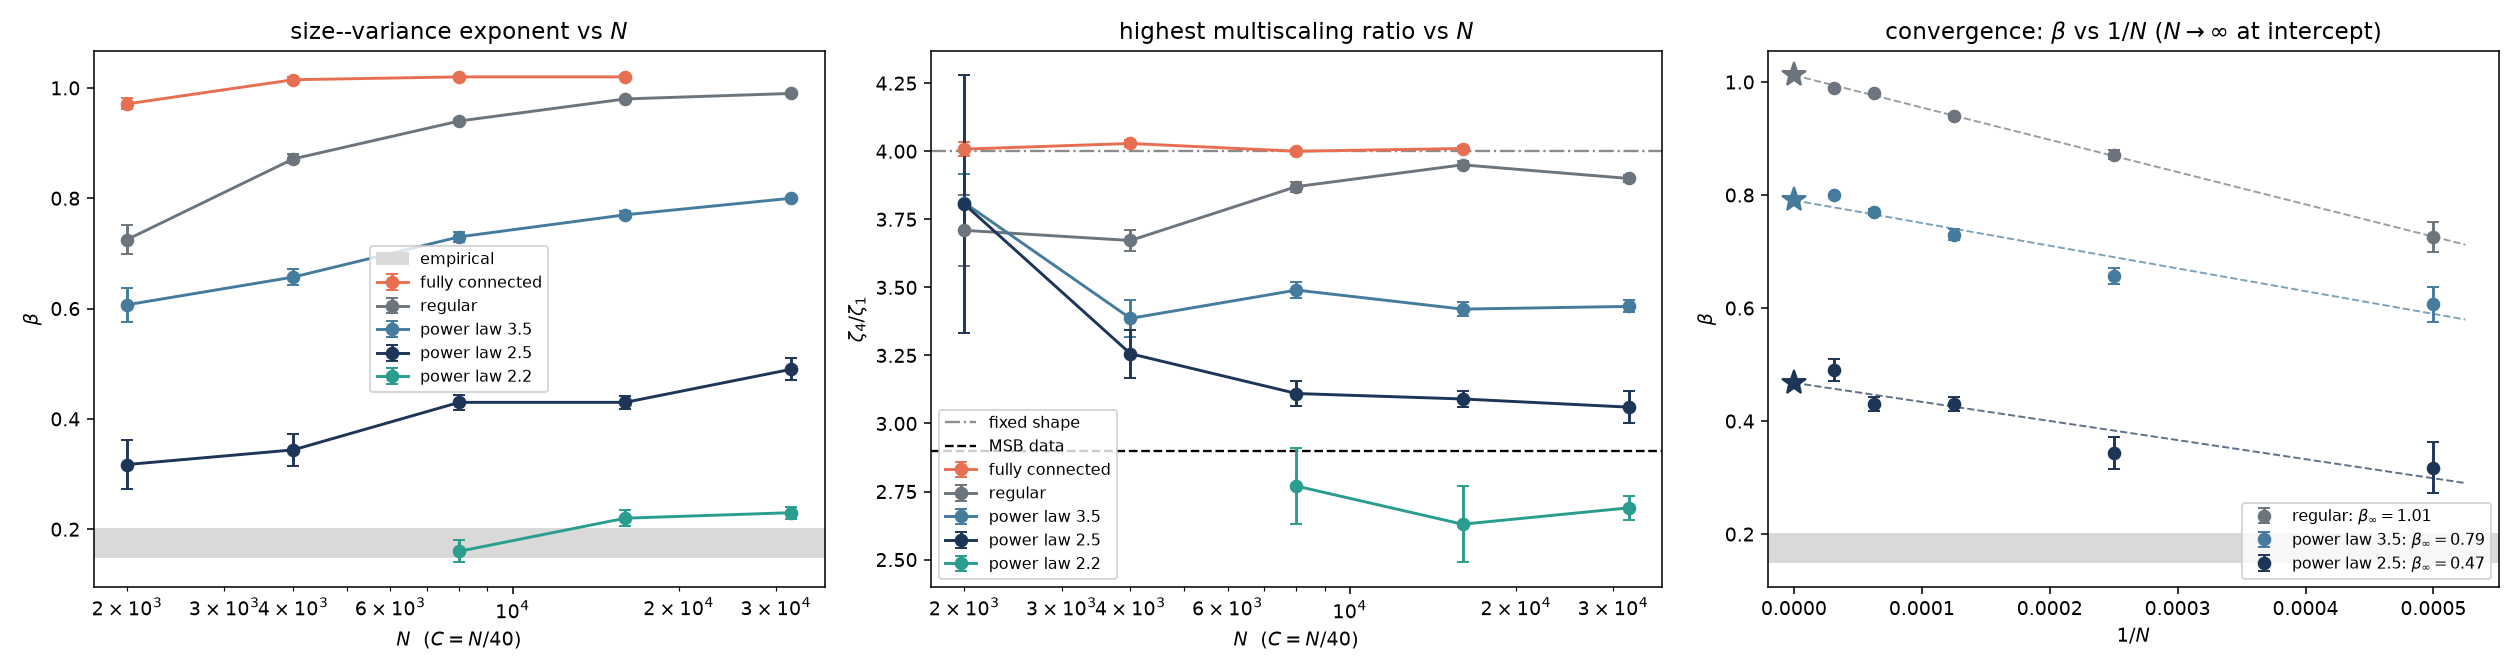
\includegraphics[width=\linewidth]{meandeg_scaling_topology.png}
    \caption{Finite-size scaling of the exponents at fixed dilution $C = N/40$, for the five
    degree distributions of Section~\ref{sec:growing-graph} (12--20 economies per point).
    \panel{Left}: the size--variance exponent $\beta$ against $N$; it drifts upward for every
    topology, but the drift shrinks and the value falls as the degree distribution broadens,
    from $\beta \approx 1$ on the homogeneous graphs to $\beta \approx 0.23$, converged, on the
    power-law-$2.2$ graph, just above the empirical band. \panel{Right}: the highest
    multiscaling ratio $\zeta_4/\zeta_1$ against $N$; flat in $N$ for every topology, set by the
    degree distribution, with the empirical value bracketed between the power-law-$2.5$ and
    power-law-$2.2$ graphs. The fully-connected graph, dense, is not run beyond $N = 16000$.}
    \label{fig:scaling-topology}
\end{figure}

\begin{table}[htbp]
    \centering
    \begin{tabular}{llccc}
        \hline
        & & $N=8000$ & $N=16000$ & $N=32000$ \\
        \hline
        \multirow{5}{*}{$\beta$}
          & fully connected & $1.02$ & $1.02$ & n/a \\
          & regular         & $0.94$ & $0.98$ & $0.99$ \\
          & power law $3.5$ & $0.73$ & $0.77$ & $0.80$ \\
          & power law $2.5$ & $0.43$ & $0.43$ & $0.49$ \\
          & power law $2.2$ & $0.16$ & $0.22$ & $0.23$ \\
        \hline
        \multirow{5}{*}{$\zeta_4/\zeta_1$}
          & fully connected & $4.00$ & $4.01$ & n/a \\
          & regular         & $3.87$ & $3.95$ & $3.90$ \\
          & power law $3.5$ & $3.49$ & $3.42$ & $3.43$ \\
          & power law $2.5$ & $3.11$ & $3.09$ & $3.06$ \\
          & power law $2.2$ & $2.77$ & $2.63$ & $2.69$ \\
        \hline
    \end{tabular}
    \caption{The size--variance exponent $\beta$ and the highest multiscaling ratio
    $\zeta_4/\zeta_1$ against system size, at $C = N/40$, for each degree distribution
    (standard errors $\le 0.02$ on $\beta$ and $\le 0.14$ on the ratio; the empirical values are
    $\beta \approx 0.15$--$0.20$ and $\zeta_4/\zeta_1 \approx 2.9$). The ratio is flat in $N$ for
    every topology; $\beta$ drifts upward but its value is set by the degree distribution, and
    for the power-law-$2.2$ graph it has converged just above the empirical band. The
    ensembles here are independent of those behind the main-text figures; where the same
    quantity appears in both, the values agree within the quoted errors. The
    fully-connected graph is dense and is not run at $N = 32000$.}
    \label{tab:scaling}
\end{table}

\chapter{Between-firm growth correlations}
\label{app:correlations}

The granular models fail, \citet{moran2024} argue, because they lack a correlation between the
growth rates of different firms, and they conjecture that this correlation grows with firm size:
the missing ingredient is that ``the correlation of a firm's growth rate with that of the whole
economy and the correlation of the growth rate of firms of similar sizes clearly grow with their
size''. The body of this thesis reproduces the size-conditioned statistics through the degree
heterogeneity of the interaction graph. That leaves a direct question, which this appendix
settles: does the model reproduce the empirical facts by the route \citet{moran2024} conjecture,
through correlations that grow with size, or by another?

We measure two correlations from the per-firm growth time series $g_i(t) = \Delta \ln S_i$ in the
fluctuating state, on the thesis graph (power-law $2.5$, mean degree $C = N/40$, $N = 16000$, ten
economies). The first is the co-movement of a firm with the aggregate,
$\rho_i = \mathrm{corr}_t\!\big(g_i(t),\,\bar g(t)\big)$, where $\bar g(t)$ is the
cross-sectional mean growth: it measures how strongly a firm tracks the common motion of the
economy. The second is the mean pairwise correlation
$\mathrm{corr}_t\!\big(g_i(t),\,g_j(t)\big)$ among firms that fall in the same bin, the direct
analogue of \citet{moran2024}'s ``correlation of firms of similar sizes''. Each is binned both by
firm size and by degree.

Both correlations are small and, to the precision reached here, flat
(Figure~\ref{fig:correlations}). The co-movement with the aggregate sits at $\rho \approx 0.09$
and is independent of size and of degree across the ranges resolved. The same-bin pairwise
correlation is an order of magnitude smaller, $\approx 0.01$, also flat, with at most a weak rise
to $\approx 0.018$ among the very largest firms. The correlations \citet{moran2024} name are thus
present but modest, and they do not grow appreciably with either size or degree.

The model therefore reproduces the size-conditioned anomalies \emph{without} the size-growing
correlations \citet{moran2024} conjecture. Its mechanism is instead the degree-dependence of the
noise \emph{amplitude}: under the dilute normalization a firm's own idiosyncratic noise variance
grows with its connectivity (Section~\ref{sec:growing-graph}), a single-firm property, riding on a
flat and modest between-firm correlation background. The model is in this sense an alternative to
\citet{moran2024}'s hypothesis rather than a realization of it: the anomalies need not come from
correlations that strengthen with size.

Two limits qualify the null result. The pairwise measure averages over same-bin pairs that are
almost all unconnected on the sparse graph, so it understates the correlation between direct
trading partners, which a production-network reading of the model would emphasize. And the
survival mechanism of Section~\ref{sec:growing-degree-size} removes the extreme hubs from the
fluctuating state: the live-firm degree axis reaches only $k \approx 470$ although the graph's
tail extends beyond $k \approx 3000$, so the most connected firms, where any correlation would be
strongest, are absent from the measurement. A direct test on firm-level data with a known
interaction network, where both restrictions could be lifted, remains open.

\begin{figure}[htbp]
    \centering
    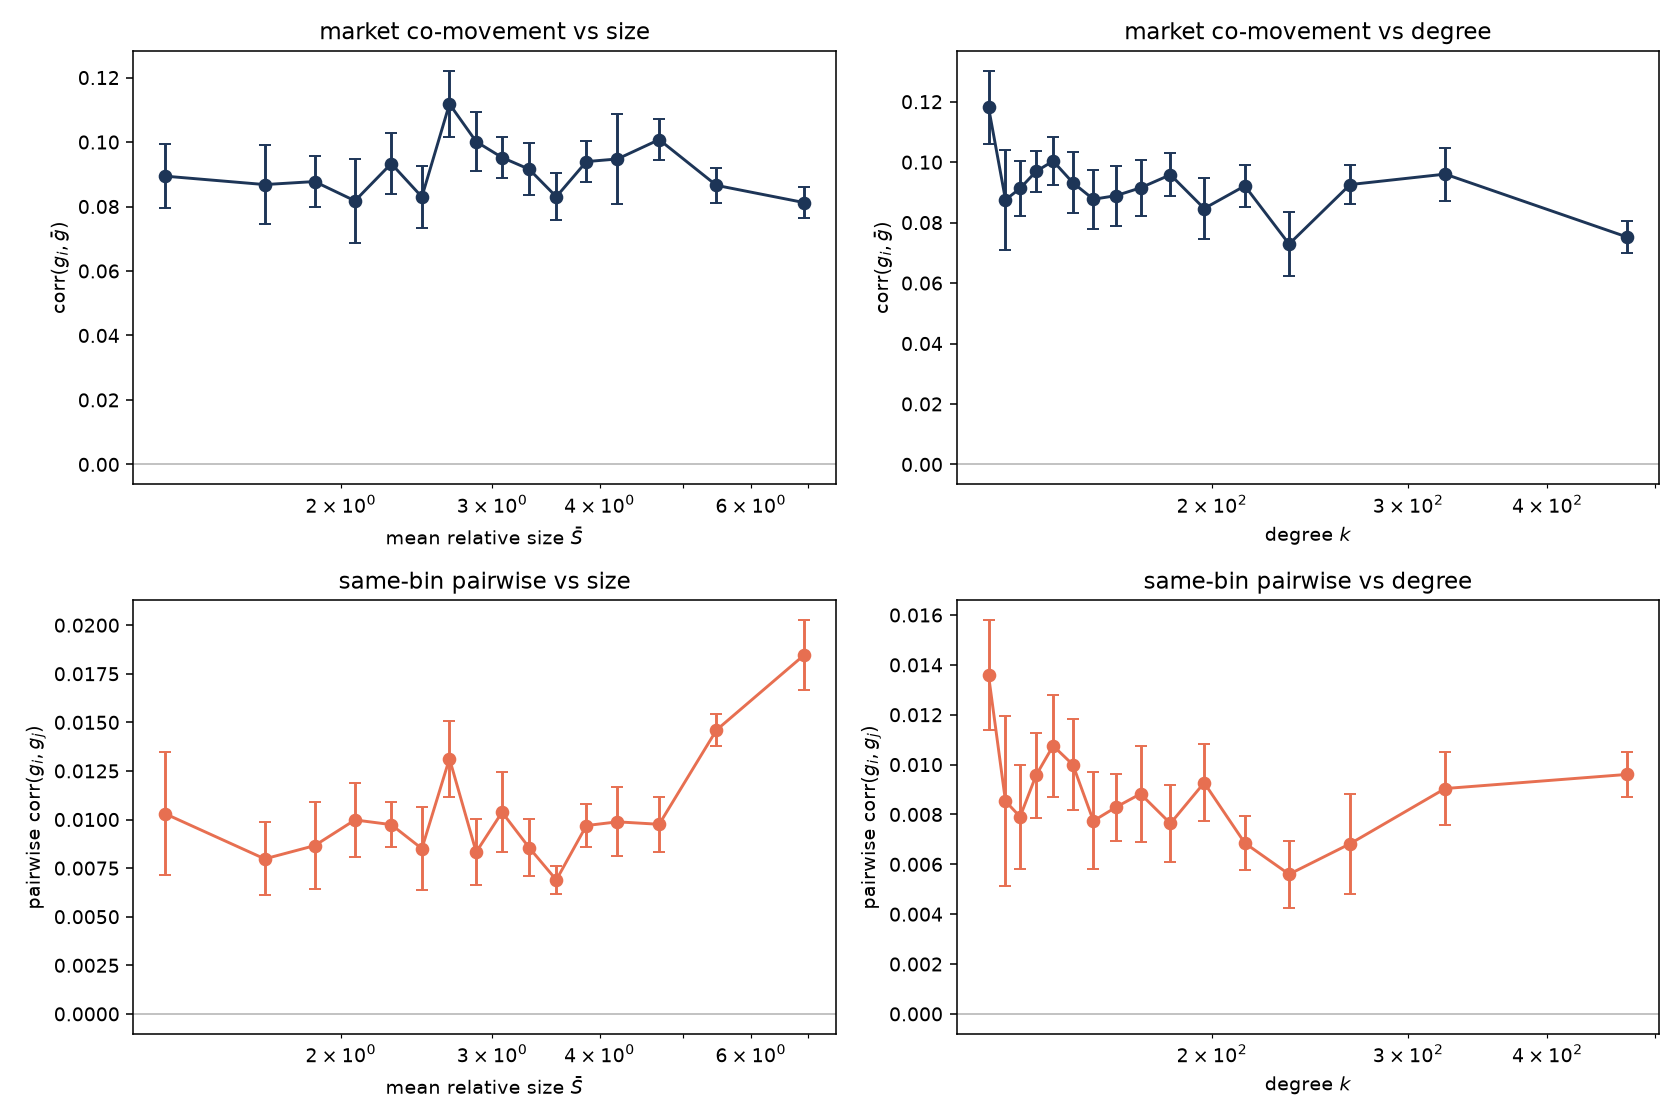
\includegraphics[width=\linewidth]{between_firm_corr.png}
    \caption{Between-firm growth correlations in the fluctuating state
    ($N = 16000$, ten economies, power-law-$2.5$ graph). \panel{Top}: the co-movement of each
    firm with the aggregate, $\mathrm{corr}(g_i, \bar g)$, against firm size (left) and degree
    (right); flat at $\approx 0.09$ on both axes. \panel{Bottom}: the mean pairwise correlation
    among firms in a bin, against size (left) and degree (right); flat at $\approx 0.01$, with a
    weak rise among the largest firms. Neither correlation grows appreciably with size or degree,
    so the model reproduces the size-conditioned statistics through the degree-dependent noise
    amplitude rather than through the size-growing correlations of \citet{moran2024}.}
    \label{fig:correlations}
\end{figure}

\chapter{Survival and re-entry dynamics}
\label{app:survival}

The selection mechanism of Section~\ref{sec:growing-degree-size} can be measured directly rather
than inferred from the survivor-size relation. Figure~\ref{fig:survival-degree} shows the
conditional survival probability for ten independent power-law-$2.5$ economies of $N = 10000$,
with $C=N/40=250$, at the operating point of the main text. A firm counts as a survivor when its
share remains above $10^{-6}$ throughout the late window $t\in[180,240]$. We calculate a rate in
each degree bin within each economy and then average the ten rates with equal weight. The bands
are $95\%$ $t$ intervals across economies, not intervals from a pooled supergraph.

Survival falls sharply with degree: the rate is $0.159\pm0.049$ in the lowest resolved bin
($k\approx75$), $0.044\pm0.015$ at $k\approx352$, and $0.014\pm0.008$ at
$k\approx985$; no survivor is observed above $k\approx2760$. This is the direct selection step
behind the degree--size relation: connectivity broadens the disorder field but competition removes
the typical high-degree firm. The graph construction itself has no sampled degrees below $k=58$,
so the figure makes no claim about a distinct low-degree network ensemble.

\begin{figure}[htbp]
    \centering
    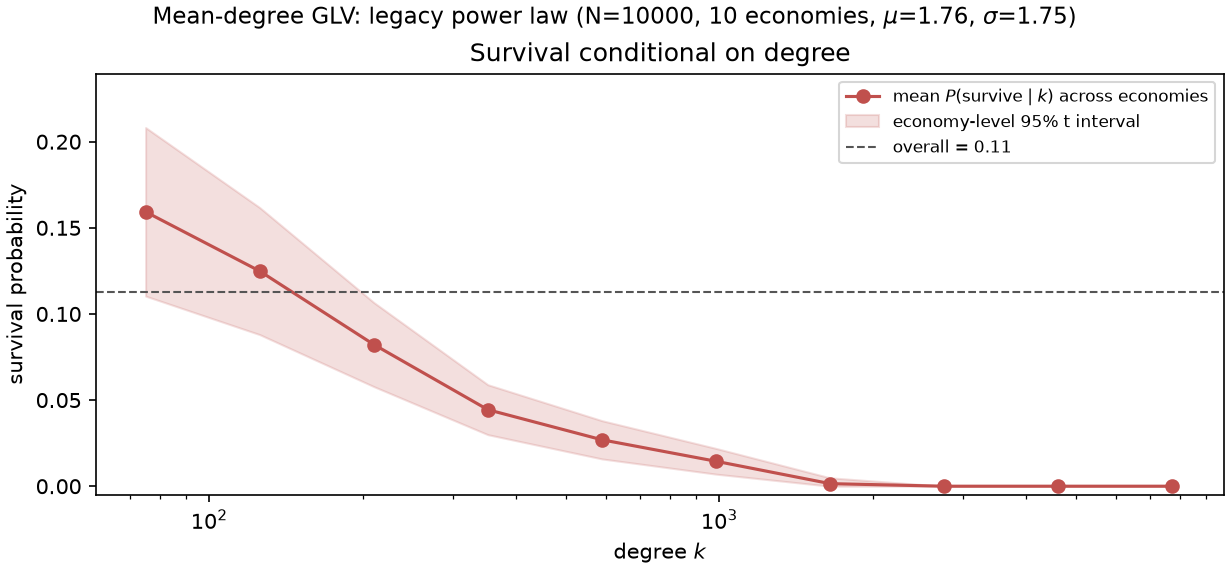
\includegraphics[width=\linewidth]{survival_by_degree.png}
    \caption{Survival conditional on degree in the thesis mean-degree power-law ensemble
    ($N=10000$, $C=250$, ten economies, $\mu=1.76$, $\sigma=1.75$). Each point is the unweighted
    mean of the within-economy survival probabilities; shading is the $95\%$ interval across
    economies. A firm is counted as surviving only if its share stays above $10^{-6}$ throughout
    $t\in[180,240]$. The probability falls steadily across the resolved support, directly exposing
    the competitive selection of hubs.}
    \label{fig:survival-degree}
\end{figure}

Crossing the threshold is not an absorbing extinction event. In the same ten trajectories we
classify a re-entry only when a firm is active, drops below the threshold, and later returns above
it; a first activation does not count. Although
only $11.3\%$ of firms remain above the threshold throughout the whole window, $87.5\%$ are active
at some point. Among firms that exit at least once, $85.4\%$ re-enter before the window ends
(Figure~\ref{fig:reentry-degree}). The re-entry probability conditional on an exit is $0.87$ in
the lowest resolved degree bin and remains $0.77$ at $k\approx985$, falling only in the
sparsely populated extreme tail. The low persistent-survival probability therefore records
turnover around the threshold rather than irreversible firm loss. Immigration continually reseeds
low shares, while the fluctuating interaction field can return a firm to the active set.

\begin{figure}[htbp]
    \centering
    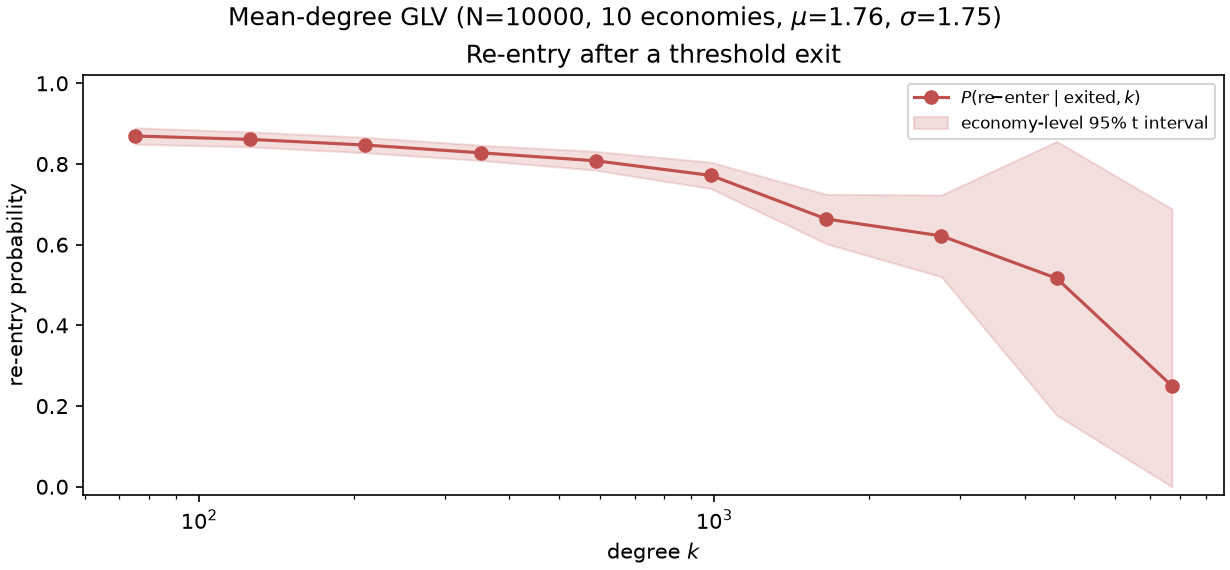
\includegraphics[width=\linewidth]{reentry_by_degree.png}
    \caption{Re-entry after a threshold exit in the thesis mean-degree power-law ensemble
    ($N=10000$, $C=250$, ten economies, $\mu=1.76$, $\sigma=1.75$). A re-entry requires an
    active--inactive--active sequence within $t\in[180,240]$; first activation is excluded.
    Each point is the unweighted mean of the within-economy probability
    $P(\mathrm{re\!\!\! - \! enter}\mid\mathrm{exited},k)$, with $95\%$ intervals across
    economies. The high re-entry rate makes explicit that threshold exits are churn, not
    absorbing extinctions.}
    \label{fig:reentry-degree}
\end{figure}

\chapter{Firm-size distribution}
\label{app:size-distribution}

Figure~\ref{fig:size-distribution} measures the stationary distribution of relative sizes
$S_i=Nw_i$ at the operating point: ten independent $N=10000$ economies, each observed over the
late window $t\in[180,240]$. The left panel keeps every observation; its lower plateau is set by the
immigration floor. The reporting cut $S=0.1$, applied only in the upper-tail panel, removes this
floor-dominated region and is not a graph cutoff. On log--log axes the active-firm tail bends
sharply instead of following a straight Pareto segment. A fit of the complementary-tail exponent
in each economy, from its upper $2\%$ of active observations, gives $\hat\mu=4.40$ with a $95\%$
$t$ interval $[4.02,4.78]$; a Zipf tail has exponent near one. The upper tail at this operating
point is far thinner, effectively truncated.

The main results of the thesis are therefore claims about the size-conditioned growth
fluctuations and their network origin, not about the cross-sectional size distribution,
which the model at this operating point does not reproduce.

\begin{figure}[!htb]
    \centering
    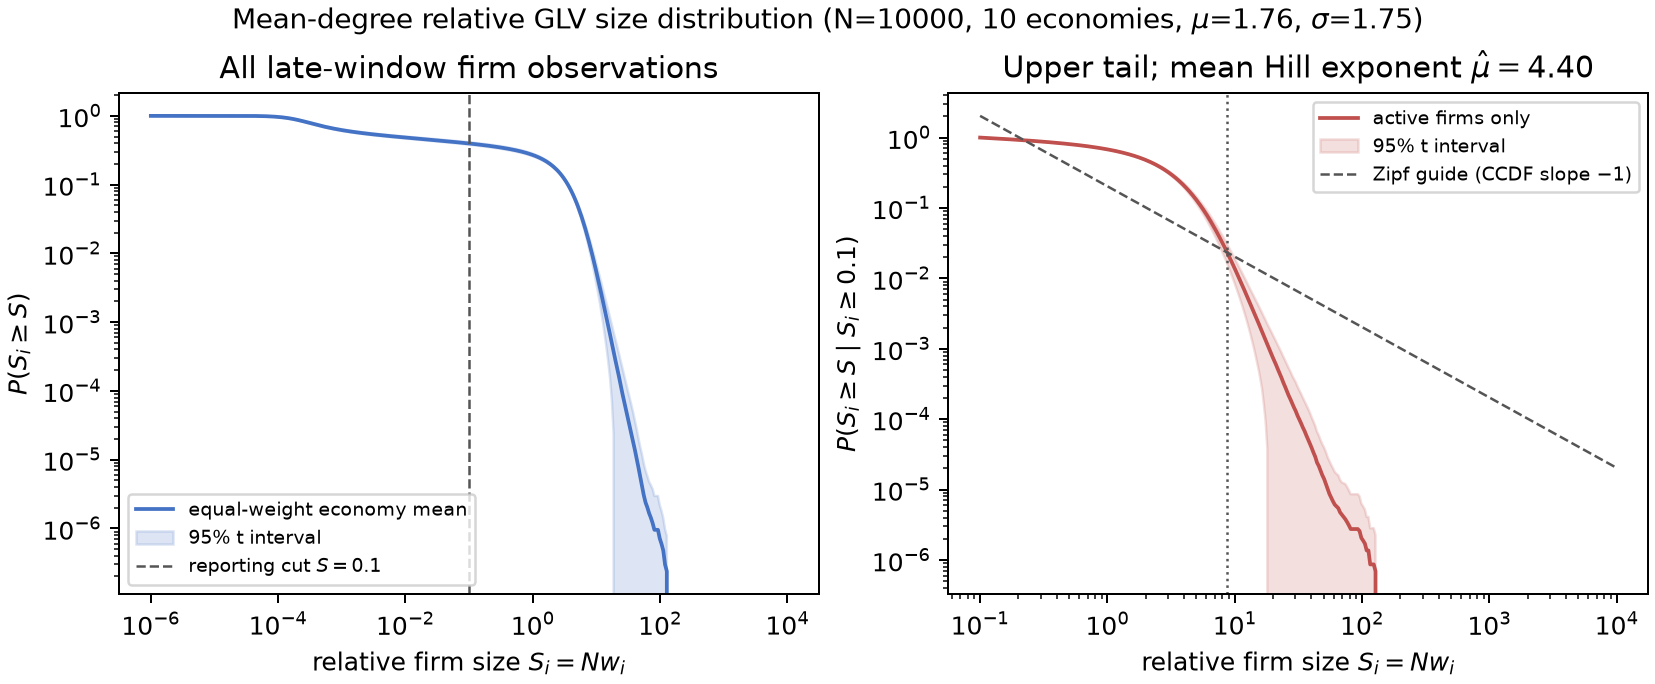
\includegraphics[width=0.82\linewidth]{size_distribution_N10000.png}
    \caption{Stationary relative firm-size distribution in the mean-degree power-law
    ensemble ($N=10000$, $C=250$, ten economies, $\mu=-1.76$, $\sigma=1.75$). Curves are
    equal-weight means of economy-level complementary distribution functions; shading is the
    $95\%$ interval across economies. \panel{Left}: all late-window observations.
    \panel{Right}: conditional upper tail of active firms, with strong curvature and a
    complementary-tail exponent near $4.4$ against the Zipf benchmark near $1$.}
    \label{fig:size-distribution}
\end{figure}

\chapter{Numerical methods and measurement protocol}
\label{app:numerics}

\section{Integration}

The relative model is integrated in physical time, the composition kept in its bounded
variables and the scale carried in its logarithm, so that nothing overflows
however large the economy becomes. Internally the solver evolves the shares
$w_i = S_i/N$, which live on the probability simplex and are renormalized onto it at
each output time; we integrate \eqref{eq:replicator} in this form
together with $\mathrm{d}\ln m/\mathrm{d}t = g_{\mathrm{eff}}$ with an explicit
Runge--Kutta solver throughout. At the system sizes reached in the text ($N$ up to
$3.2\times10^4$) the implicit solvers tried first switched to a dense Jacobian and became
prohibitively slow, whereas the explicit method integrates one run to $t = 250$ in about
ten seconds at $N = 10^4$.

\section{Volatility estimator}

The per-firm growth-rate volatility is measured with the mean-absolute-deviation
estimator
\begin{equation}
    \sigma_i = \sqrt{\tfrac{\pi}{2}}\,\big\langle\, \big|\,g_i - \langle g_i\rangle\,\big| \,\big\rangle ,
\end{equation}
rescaled by the Gaussian-consistent factor $\sqrt{\pi/2}$ and used in place of the
standard deviation for robustness against the fat tails of the growth rates.

\section{Size--volatility fit}

The immigration floor makes the smallest firms quiet, producing a plateau at the bottom
of the size range. The size--volatility relation $\sigma(\bar S)$ is therefore fitted
only over its power-law range, the monotone decline above that plateau, and we report the
coefficient of determination $R^2$ of the fit rather than forcing a single slope across a
shape that is not a power law. The exponent quoted in the text, $\beta = 0.45 \pm 0.06$, is
the median and economy-to-economy standard deviation of this decline-branch slope over
twenty independent disorder realizations at $N = 16000$; the spread is set by the disorder
realization rather than the fit, whose pooled-decline $R^2$ is $0.99$. All exponents,
including the higher moments $\zeta_q$, are fitted per economy and averaged
(Section~\ref{sec:growing-estimator}); pooled fits are quoted only for comparison.

\section{Code availability}

The model, the measurement protocols described above, and a generator for every
reproducible figure in this thesis are available at
\url{https://github.com/NotLudovico/dynamical-model-for-economics}. The repository
includes the dynamical mean-field solver of Appendix~\ref{app:dmft} and its validation
against direct simulation.


\end{document}
